
% Default to the notebook output style

    


% Inherit from the specified cell style.




    
\documentclass[11pt]{article}

    
    
    \usepackage[T1]{fontenc}
    % Nicer default font than Computer Modern for most use cases
    \usepackage{palatino}

    % Basic figure setup, for now with no caption control since it's done
    % automatically by Pandoc (which extracts ![](path) syntax from Markdown).
    \usepackage{graphicx}
    % We will generate all images so they have a width \maxwidth. This means
    % that they will get their normal width if they fit onto the page, but
    % are scaled down if they would overflow the margins.
    \makeatletter
    \def\maxwidth{\ifdim\Gin@nat@width>\linewidth\linewidth
    \else\Gin@nat@width\fi}
    \makeatother
    \let\Oldincludegraphics\includegraphics
    % Set max figure width to be 80% of text width, for now hardcoded.
    \renewcommand{\includegraphics}[1]{\Oldincludegraphics[width=.8\maxwidth]{#1}}
    % Ensure that by default, figures have no caption (until we provide a
    % proper Figure object with a Caption API and a way to capture that
    % in the conversion process - todo).
    \usepackage{caption}
    \DeclareCaptionLabelFormat{nolabel}{}
    \captionsetup{labelformat=nolabel}

    \usepackage{adjustbox} % Used to constrain images to a maximum size 
    \usepackage{xcolor} % Allow colors to be defined
    \usepackage{enumerate} % Needed for markdown enumerations to work
    \usepackage{geometry} % Used to adjust the document margins
    \usepackage{amsmath} % Equations
    \usepackage{amssymb} % Equations
    \usepackage{textcomp} % defines textquotesingle
    % Hack from http://tex.stackexchange.com/a/47451/13684:
    \AtBeginDocument{%
        \def\PYZsq{\textquotesingle}% Upright quotes in Pygmentized code
    }
    \usepackage{upquote} % Upright quotes for verbatim code
    \usepackage{eurosym} % defines \euro
    \usepackage[mathletters]{ucs} % Extended unicode (utf-8) support
    \usepackage[utf8x]{inputenc} % Allow utf-8 characters in the tex document
    \usepackage{fancyvrb} % verbatim replacement that allows latex
    \usepackage{grffile} % extends the file name processing of package graphics 
                         % to support a larger range 
    % The hyperref package gives us a pdf with properly built
    % internal navigation ('pdf bookmarks' for the table of contents,
    % internal cross-reference links, web links for URLs, etc.)
    \usepackage{hyperref}
    \usepackage{longtable} % longtable support required by pandoc >1.10
    \usepackage{booktabs}  % table support for pandoc > 1.12.2
    \usepackage[normalem]{ulem} % ulem is needed to support strikethroughs (\sout)
                                % normalem makes italics be italics, not underlines
    

    
    
    % Colors for the hyperref package
    \definecolor{urlcolor}{rgb}{0,.145,.698}
    \definecolor{linkcolor}{rgb}{.71,0.21,0.01}
    \definecolor{citecolor}{rgb}{.12,.54,.11}

    % ANSI colors
    \definecolor{ansi-black}{HTML}{3E424D}
    \definecolor{ansi-black-intense}{HTML}{282C36}
    \definecolor{ansi-red}{HTML}{E75C58}
    \definecolor{ansi-red-intense}{HTML}{B22B31}
    \definecolor{ansi-green}{HTML}{00A250}
    \definecolor{ansi-green-intense}{HTML}{007427}
    \definecolor{ansi-yellow}{HTML}{DDB62B}
    \definecolor{ansi-yellow-intense}{HTML}{B27D12}
    \definecolor{ansi-blue}{HTML}{208FFB}
    \definecolor{ansi-blue-intense}{HTML}{0065CA}
    \definecolor{ansi-magenta}{HTML}{D160C4}
    \definecolor{ansi-magenta-intense}{HTML}{A03196}
    \definecolor{ansi-cyan}{HTML}{60C6C8}
    \definecolor{ansi-cyan-intense}{HTML}{258F8F}
    \definecolor{ansi-white}{HTML}{C5C1B4}
    \definecolor{ansi-white-intense}{HTML}{A1A6B2}

    % commands and environments needed by pandoc snippets
    % extracted from the output of `pandoc -s`
    \providecommand{\tightlist}{%
      \setlength{\itemsep}{0pt}\setlength{\parskip}{0pt}}
    \DefineVerbatimEnvironment{Highlighting}{Verbatim}{commandchars=\\\{\}}
    % Add ',fontsize=\small' for more characters per line
    \newenvironment{Shaded}{}{}
    \newcommand{\KeywordTok}[1]{\textcolor[rgb]{0.00,0.44,0.13}{\textbf{{#1}}}}
    \newcommand{\DataTypeTok}[1]{\textcolor[rgb]{0.56,0.13,0.00}{{#1}}}
    \newcommand{\DecValTok}[1]{\textcolor[rgb]{0.25,0.63,0.44}{{#1}}}
    \newcommand{\BaseNTok}[1]{\textcolor[rgb]{0.25,0.63,0.44}{{#1}}}
    \newcommand{\FloatTok}[1]{\textcolor[rgb]{0.25,0.63,0.44}{{#1}}}
    \newcommand{\CharTok}[1]{\textcolor[rgb]{0.25,0.44,0.63}{{#1}}}
    \newcommand{\StringTok}[1]{\textcolor[rgb]{0.25,0.44,0.63}{{#1}}}
    \newcommand{\CommentTok}[1]{\textcolor[rgb]{0.38,0.63,0.69}{\textit{{#1}}}}
    \newcommand{\OtherTok}[1]{\textcolor[rgb]{0.00,0.44,0.13}{{#1}}}
    \newcommand{\AlertTok}[1]{\textcolor[rgb]{1.00,0.00,0.00}{\textbf{{#1}}}}
    \newcommand{\FunctionTok}[1]{\textcolor[rgb]{0.02,0.16,0.49}{{#1}}}
    \newcommand{\RegionMarkerTok}[1]{{#1}}
    \newcommand{\ErrorTok}[1]{\textcolor[rgb]{1.00,0.00,0.00}{\textbf{{#1}}}}
    \newcommand{\NormalTok}[1]{{#1}}
    
    % Additional commands for more recent versions of Pandoc
    \newcommand{\ConstantTok}[1]{\textcolor[rgb]{0.53,0.00,0.00}{{#1}}}
    \newcommand{\SpecialCharTok}[1]{\textcolor[rgb]{0.25,0.44,0.63}{{#1}}}
    \newcommand{\VerbatimStringTok}[1]{\textcolor[rgb]{0.25,0.44,0.63}{{#1}}}
    \newcommand{\SpecialStringTok}[1]{\textcolor[rgb]{0.73,0.40,0.53}{{#1}}}
    \newcommand{\ImportTok}[1]{{#1}}
    \newcommand{\DocumentationTok}[1]{\textcolor[rgb]{0.73,0.13,0.13}{\textit{{#1}}}}
    \newcommand{\AnnotationTok}[1]{\textcolor[rgb]{0.38,0.63,0.69}{\textbf{\textit{{#1}}}}}
    \newcommand{\CommentVarTok}[1]{\textcolor[rgb]{0.38,0.63,0.69}{\textbf{\textit{{#1}}}}}
    \newcommand{\VariableTok}[1]{\textcolor[rgb]{0.10,0.09,0.49}{{#1}}}
    \newcommand{\ControlFlowTok}[1]{\textcolor[rgb]{0.00,0.44,0.13}{\textbf{{#1}}}}
    \newcommand{\OperatorTok}[1]{\textcolor[rgb]{0.40,0.40,0.40}{{#1}}}
    \newcommand{\BuiltInTok}[1]{{#1}}
    \newcommand{\ExtensionTok}[1]{{#1}}
    \newcommand{\PreprocessorTok}[1]{\textcolor[rgb]{0.74,0.48,0.00}{{#1}}}
    \newcommand{\AttributeTok}[1]{\textcolor[rgb]{0.49,0.56,0.16}{{#1}}}
    \newcommand{\InformationTok}[1]{\textcolor[rgb]{0.38,0.63,0.69}{\textbf{\textit{{#1}}}}}
    \newcommand{\WarningTok}[1]{\textcolor[rgb]{0.38,0.63,0.69}{\textbf{\textit{{#1}}}}}
    
    
    % Define a nice break command that doesn't care if a line doesn't already
    % exist.
    \def\br{\hspace*{\fill} \\* }
    % Math Jax compatability definitions
    \def\gt{>}
    \def\lt{<}
    % Document parameters
    \title{p}
    
    
    

    % Pygments definitions
    
\makeatletter
\def\PY@reset{\let\PY@it=\relax \let\PY@bf=\relax%
    \let\PY@ul=\relax \let\PY@tc=\relax%
    \let\PY@bc=\relax \let\PY@ff=\relax}
\def\PY@tok#1{\csname PY@tok@#1\endcsname}
\def\PY@toks#1+{\ifx\relax#1\empty\else%
    \PY@tok{#1}\expandafter\PY@toks\fi}
\def\PY@do#1{\PY@bc{\PY@tc{\PY@ul{%
    \PY@it{\PY@bf{\PY@ff{#1}}}}}}}
\def\PY#1#2{\PY@reset\PY@toks#1+\relax+\PY@do{#2}}

\expandafter\def\csname PY@tok@gd\endcsname{\def\PY@tc##1{\textcolor[rgb]{0.63,0.00,0.00}{##1}}}
\expandafter\def\csname PY@tok@gu\endcsname{\let\PY@bf=\textbf\def\PY@tc##1{\textcolor[rgb]{0.50,0.00,0.50}{##1}}}
\expandafter\def\csname PY@tok@gt\endcsname{\def\PY@tc##1{\textcolor[rgb]{0.00,0.27,0.87}{##1}}}
\expandafter\def\csname PY@tok@gs\endcsname{\let\PY@bf=\textbf}
\expandafter\def\csname PY@tok@gr\endcsname{\def\PY@tc##1{\textcolor[rgb]{1.00,0.00,0.00}{##1}}}
\expandafter\def\csname PY@tok@cm\endcsname{\let\PY@it=\textit\def\PY@tc##1{\textcolor[rgb]{0.25,0.50,0.50}{##1}}}
\expandafter\def\csname PY@tok@vg\endcsname{\def\PY@tc##1{\textcolor[rgb]{0.10,0.09,0.49}{##1}}}
\expandafter\def\csname PY@tok@vi\endcsname{\def\PY@tc##1{\textcolor[rgb]{0.10,0.09,0.49}{##1}}}
\expandafter\def\csname PY@tok@mh\endcsname{\def\PY@tc##1{\textcolor[rgb]{0.40,0.40,0.40}{##1}}}
\expandafter\def\csname PY@tok@cs\endcsname{\let\PY@it=\textit\def\PY@tc##1{\textcolor[rgb]{0.25,0.50,0.50}{##1}}}
\expandafter\def\csname PY@tok@ge\endcsname{\let\PY@it=\textit}
\expandafter\def\csname PY@tok@vc\endcsname{\def\PY@tc##1{\textcolor[rgb]{0.10,0.09,0.49}{##1}}}
\expandafter\def\csname PY@tok@il\endcsname{\def\PY@tc##1{\textcolor[rgb]{0.40,0.40,0.40}{##1}}}
\expandafter\def\csname PY@tok@go\endcsname{\def\PY@tc##1{\textcolor[rgb]{0.53,0.53,0.53}{##1}}}
\expandafter\def\csname PY@tok@cp\endcsname{\def\PY@tc##1{\textcolor[rgb]{0.74,0.48,0.00}{##1}}}
\expandafter\def\csname PY@tok@gi\endcsname{\def\PY@tc##1{\textcolor[rgb]{0.00,0.63,0.00}{##1}}}
\expandafter\def\csname PY@tok@gh\endcsname{\let\PY@bf=\textbf\def\PY@tc##1{\textcolor[rgb]{0.00,0.00,0.50}{##1}}}
\expandafter\def\csname PY@tok@ni\endcsname{\let\PY@bf=\textbf\def\PY@tc##1{\textcolor[rgb]{0.60,0.60,0.60}{##1}}}
\expandafter\def\csname PY@tok@nl\endcsname{\def\PY@tc##1{\textcolor[rgb]{0.63,0.63,0.00}{##1}}}
\expandafter\def\csname PY@tok@nn\endcsname{\let\PY@bf=\textbf\def\PY@tc##1{\textcolor[rgb]{0.00,0.00,1.00}{##1}}}
\expandafter\def\csname PY@tok@no\endcsname{\def\PY@tc##1{\textcolor[rgb]{0.53,0.00,0.00}{##1}}}
\expandafter\def\csname PY@tok@na\endcsname{\def\PY@tc##1{\textcolor[rgb]{0.49,0.56,0.16}{##1}}}
\expandafter\def\csname PY@tok@nb\endcsname{\def\PY@tc##1{\textcolor[rgb]{0.00,0.50,0.00}{##1}}}
\expandafter\def\csname PY@tok@nc\endcsname{\let\PY@bf=\textbf\def\PY@tc##1{\textcolor[rgb]{0.00,0.00,1.00}{##1}}}
\expandafter\def\csname PY@tok@nd\endcsname{\def\PY@tc##1{\textcolor[rgb]{0.67,0.13,1.00}{##1}}}
\expandafter\def\csname PY@tok@ne\endcsname{\let\PY@bf=\textbf\def\PY@tc##1{\textcolor[rgb]{0.82,0.25,0.23}{##1}}}
\expandafter\def\csname PY@tok@nf\endcsname{\def\PY@tc##1{\textcolor[rgb]{0.00,0.00,1.00}{##1}}}
\expandafter\def\csname PY@tok@si\endcsname{\let\PY@bf=\textbf\def\PY@tc##1{\textcolor[rgb]{0.73,0.40,0.53}{##1}}}
\expandafter\def\csname PY@tok@s2\endcsname{\def\PY@tc##1{\textcolor[rgb]{0.73,0.13,0.13}{##1}}}
\expandafter\def\csname PY@tok@nt\endcsname{\let\PY@bf=\textbf\def\PY@tc##1{\textcolor[rgb]{0.00,0.50,0.00}{##1}}}
\expandafter\def\csname PY@tok@nv\endcsname{\def\PY@tc##1{\textcolor[rgb]{0.10,0.09,0.49}{##1}}}
\expandafter\def\csname PY@tok@s1\endcsname{\def\PY@tc##1{\textcolor[rgb]{0.73,0.13,0.13}{##1}}}
\expandafter\def\csname PY@tok@ch\endcsname{\let\PY@it=\textit\def\PY@tc##1{\textcolor[rgb]{0.25,0.50,0.50}{##1}}}
\expandafter\def\csname PY@tok@m\endcsname{\def\PY@tc##1{\textcolor[rgb]{0.40,0.40,0.40}{##1}}}
\expandafter\def\csname PY@tok@gp\endcsname{\let\PY@bf=\textbf\def\PY@tc##1{\textcolor[rgb]{0.00,0.00,0.50}{##1}}}
\expandafter\def\csname PY@tok@sh\endcsname{\def\PY@tc##1{\textcolor[rgb]{0.73,0.13,0.13}{##1}}}
\expandafter\def\csname PY@tok@ow\endcsname{\let\PY@bf=\textbf\def\PY@tc##1{\textcolor[rgb]{0.67,0.13,1.00}{##1}}}
\expandafter\def\csname PY@tok@sx\endcsname{\def\PY@tc##1{\textcolor[rgb]{0.00,0.50,0.00}{##1}}}
\expandafter\def\csname PY@tok@bp\endcsname{\def\PY@tc##1{\textcolor[rgb]{0.00,0.50,0.00}{##1}}}
\expandafter\def\csname PY@tok@c1\endcsname{\let\PY@it=\textit\def\PY@tc##1{\textcolor[rgb]{0.25,0.50,0.50}{##1}}}
\expandafter\def\csname PY@tok@o\endcsname{\def\PY@tc##1{\textcolor[rgb]{0.40,0.40,0.40}{##1}}}
\expandafter\def\csname PY@tok@kc\endcsname{\let\PY@bf=\textbf\def\PY@tc##1{\textcolor[rgb]{0.00,0.50,0.00}{##1}}}
\expandafter\def\csname PY@tok@c\endcsname{\let\PY@it=\textit\def\PY@tc##1{\textcolor[rgb]{0.25,0.50,0.50}{##1}}}
\expandafter\def\csname PY@tok@mf\endcsname{\def\PY@tc##1{\textcolor[rgb]{0.40,0.40,0.40}{##1}}}
\expandafter\def\csname PY@tok@err\endcsname{\def\PY@bc##1{\setlength{\fboxsep}{0pt}\fcolorbox[rgb]{1.00,0.00,0.00}{1,1,1}{\strut ##1}}}
\expandafter\def\csname PY@tok@mb\endcsname{\def\PY@tc##1{\textcolor[rgb]{0.40,0.40,0.40}{##1}}}
\expandafter\def\csname PY@tok@ss\endcsname{\def\PY@tc##1{\textcolor[rgb]{0.10,0.09,0.49}{##1}}}
\expandafter\def\csname PY@tok@sr\endcsname{\def\PY@tc##1{\textcolor[rgb]{0.73,0.40,0.53}{##1}}}
\expandafter\def\csname PY@tok@mo\endcsname{\def\PY@tc##1{\textcolor[rgb]{0.40,0.40,0.40}{##1}}}
\expandafter\def\csname PY@tok@kd\endcsname{\let\PY@bf=\textbf\def\PY@tc##1{\textcolor[rgb]{0.00,0.50,0.00}{##1}}}
\expandafter\def\csname PY@tok@mi\endcsname{\def\PY@tc##1{\textcolor[rgb]{0.40,0.40,0.40}{##1}}}
\expandafter\def\csname PY@tok@kn\endcsname{\let\PY@bf=\textbf\def\PY@tc##1{\textcolor[rgb]{0.00,0.50,0.00}{##1}}}
\expandafter\def\csname PY@tok@cpf\endcsname{\let\PY@it=\textit\def\PY@tc##1{\textcolor[rgb]{0.25,0.50,0.50}{##1}}}
\expandafter\def\csname PY@tok@kr\endcsname{\let\PY@bf=\textbf\def\PY@tc##1{\textcolor[rgb]{0.00,0.50,0.00}{##1}}}
\expandafter\def\csname PY@tok@s\endcsname{\def\PY@tc##1{\textcolor[rgb]{0.73,0.13,0.13}{##1}}}
\expandafter\def\csname PY@tok@kp\endcsname{\def\PY@tc##1{\textcolor[rgb]{0.00,0.50,0.00}{##1}}}
\expandafter\def\csname PY@tok@w\endcsname{\def\PY@tc##1{\textcolor[rgb]{0.73,0.73,0.73}{##1}}}
\expandafter\def\csname PY@tok@kt\endcsname{\def\PY@tc##1{\textcolor[rgb]{0.69,0.00,0.25}{##1}}}
\expandafter\def\csname PY@tok@sc\endcsname{\def\PY@tc##1{\textcolor[rgb]{0.73,0.13,0.13}{##1}}}
\expandafter\def\csname PY@tok@sb\endcsname{\def\PY@tc##1{\textcolor[rgb]{0.73,0.13,0.13}{##1}}}
\expandafter\def\csname PY@tok@k\endcsname{\let\PY@bf=\textbf\def\PY@tc##1{\textcolor[rgb]{0.00,0.50,0.00}{##1}}}
\expandafter\def\csname PY@tok@se\endcsname{\let\PY@bf=\textbf\def\PY@tc##1{\textcolor[rgb]{0.73,0.40,0.13}{##1}}}
\expandafter\def\csname PY@tok@sd\endcsname{\let\PY@it=\textit\def\PY@tc##1{\textcolor[rgb]{0.73,0.13,0.13}{##1}}}

\def\PYZbs{\char`\\}
\def\PYZus{\char`\_}
\def\PYZob{\char`\{}
\def\PYZcb{\char`\}}
\def\PYZca{\char`\^}
\def\PYZam{\char`\&}
\def\PYZlt{\char`\<}
\def\PYZgt{\char`\>}
\def\PYZsh{\char`\#}
\def\PYZpc{\char`\%}
\def\PYZdl{\char`\$}
\def\PYZhy{\char`\-}
\def\PYZsq{\char`\'}
\def\PYZdq{\char`\"}
\def\PYZti{\char`\~}
% for compatibility with earlier versions
\def\PYZat{@}
\def\PYZlb{[}
\def\PYZrb{]}
\makeatother


    % Exact colors from NB
    \definecolor{incolor}{rgb}{0.0, 0.0, 0.5}
    \definecolor{outcolor}{rgb}{0.545, 0.0, 0.0}
    
    \usepackage[framemethod=tikz]{mdframed}



    
    % Prevent overflowing lines due to hard-to-break entities
    \sloppy 
    % Setup hyperref package
    \hypersetup{
      breaklinks=true,  % so long urls are correctly broken across lines
      colorlinks=true,
      urlcolor=urlcolor,
      linkcolor=linkcolor,
      citecolor=citecolor,
      }
    % Slightly bigger margins than the latex defaults
    
    \geometry{verbose,tmargin=1in,bmargin=1in,lmargin=1in,rmargin=1in}
    
    

    \begin{document}
    
    
    \maketitle
    
    

    
    \section{Table of Contents}\label{table-of-contents}

{1~~}Resumen teórico

{1.1~~}Definición formal

{1.2~~}Funciones kernel

{1.3~~}Outliers

{1.4~~}Preprocesado de datos

{1.4.1~~}Atributos categóricos

{1.4.2~~}Escalado

{1.5~~}Selección del modelo

{1.6~~}Cross-validation

{2~~}Notas a la implementación

{3~~}Análisis del fichero s

{3.1~~}Cargar los ficheros s-train/test

{3.2~~}Seleccionar las 3 clases más frecuentes

{3.3~~}Obtención de un clasificador MVS lineal en el espacio de
parámetros

{3.4~~}Realizar una búsqueda similar para núcleos polinómicos de grado 2

{3.5~~}Obtención de un clasificador MVS lineal en el espacio proyectado
mediante un núcleo gaussiano

{4~~}Probar distintos tipos de nucleos con un problema no separable
linealmente

{4.1~~}Gausianas con escaso solape - separables linealmente

{4.2~~}Gausianas fuertemente solapadas - no separables

{4.3~~}Gausianas separables polinómicamente

{5~~}Utilizar el resto de conjuntos y discutir los resultados

{5.1~~}Conjunto c

{5.2~~}Conjunto p

{5.3~~}Conjunto v

{5.4~~}Conjunto h

{5.5~~}Conjunto z

{5.6~~}Análisis de resultados en los conjuntos c, p, v, h y z

{6~~}Referencias

    \section{Resumen teórico}\label{resumen-teuxf3rico}

Las máquinas de soporte vectorial son un tipo de algoritmos utilizados
principalmente para clasificación y para regresión desarollados por
Vladimir Vapnik y su equipo {[}1{]}.

Las máquinas de soporte vectorial funcionan generando un hiperplano que
separa el espacio de muestras de forma que, idealmente, patrones de
diferentes clases nunca aparezcan en el mismo lado del plano. Como
existen infinitos hiperplanos que separen el espacio, se busca aquel
cuya distancia entre el hiperplano y los patrones de cada clase sea la
máxima posible (ver Figura 1). A los puntos que conforman las dos líneas
paralelas al hiperplano, siendo la distancia entre ellas (margen) la
mayor posible, se les denomina vectores de soporte. En la fase de
entrenamiento de las máquinas de soporte vectorial, nos centraremos en
hallar los vectores de soporte empleando técnicas de programación
cuadrática {[}3{]}.

Una vez obtenemos el hiperplano podemos utilizar la Máquina en problemas
de clasificación, escogiendo patrones que no hayan sido vistos durante
la fase de entrenamiento, y aplicando una etiqueta (clase) en función
del lado del hiperplano en el que se proyecten.

\begin{figure}
\centering
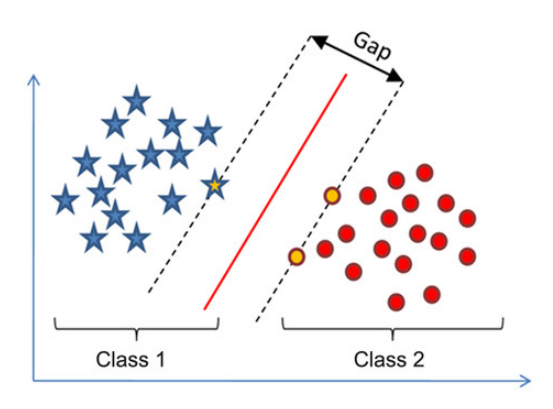
\includegraphics{esquema-basico-svm.PNG}
\caption{Figura 1: Ejemplo de 2 dimensiones para una máquina de soporte
vectorial, obsérvese que la recta roja es la que maximiza la distancia
entre los vectores de soporte (los puntos en amarillo)}
\end{figure}

Los universos a estudiar no se suelen presentar en casos idílicos de dos
dimensiones como en el ejemplo anterior, sino que un algoritmo SVM debe
tratar con:

\begin{itemize}
\tightlist
\item
  Más de dos variables predictoras
\item
  Curvas no lineales de separación
\item
  Casos donde los conjuntos de datos no pueden ser completamente
  separados
\item
  Clasificaciones en más de dos categorías
\end{itemize}

\begin{figure}
\centering
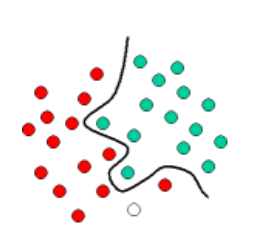
\includegraphics{no-separable-linealmente.PNG}
\caption{Figura 2: Espacio de 2 dimensiones en el que los patrones no
son separables linealmente}
\end{figure}

\subsection{Definición formal}\label{definiciuxf3n-formal}

\begin{quote}
Dado un conjunto de entrenamiento formado por pares de instancias y
etiquetas
\[(x_i,y_i),  i=1, . . . , l \text{ donde } x_i \in R^n, y \in \{1, −1\}^l\]
, las SVMs pueden entenderse como la solución al siguiente problema de
optimización:: \[
\begin{aligned}
\underset{w,b,\epsilon}{\operatorname{argmin}} & & \frac{1}{2}w^Tw + C
\sum_1^l{\epsilon_i} \\
\text{sujeto a} & & y_i(w^T \phi(x_i) + b) \ge 1- \epsilon_i \\
& & \epsilon_i \ge 0
\end{aligned}
\] Además, \[K(x_i, x_j ) ≡ \phi(x_i)^T \phi(x_j)\] es llamada la
función kernel.
\end{quote}

\emph{Figura 3. Definición formal de las SVMs según {[}4{]}}

Los vectores de entrenamiento \(x_i\) son asignados a un espacio de
mayor dimensiones (incluso infinitas) por la función \(\phi\). La
máquina de soporte vectorial encuentra el hiperplano con máximo margen
de separación en el espacio dimensional superior. C \textgreater{} 0 es
el parámetro de penalización del término de error.

\subsection{Funciones kernel}\label{funciones-kernel}

Cuando el espacio donde trabajamos no permite separar linealmente los
patrones de forma perfecta, como se puede observar en la figura 2, es
imposible trazar un hiperplano que separe perfectamente los patrones.

Por ello entran en juego las llamadas \textbf{funciones kernel},
funciones matemáticas que nos permiten proyectar los patrones en un
espacio de mayor dimensión que el original dónde estos si son
linealmente separables mediante un hiperplano (Figura 3).

\begin{figure}
\centering
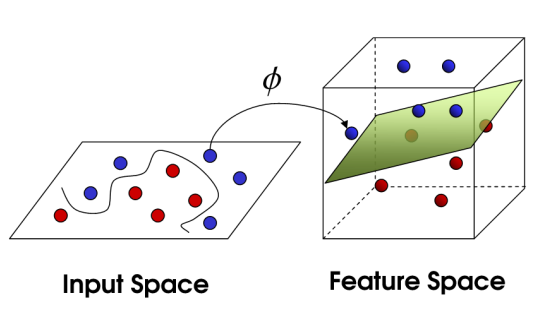
\includegraphics{ejemplo-kernel.PNG}
\caption{Figura 4: Kernel de 2 a 3 dimensiones dónde los patrones pueden
ser perfectamente separados mediante un hiperplano}
\end{figure}

De nuevo, y como en la gran mayoría de algoritmos de aprendizaje
máquina, \textbf{si elegimos un modelo (en este caso una función kernel)
que se ajuste demasiado bien a los patrones de entrenamiento}, el
clasificador perderá capacidad de generalización por lo que tendrá un
mal comportamiento ante nuevos patrones y se hablará de
\textbf{sobreentrenamiento}.

Las funciones kernel más comunmente utilizadas son:

\begin{itemize}
\tightlist
\item
  \textbf{lineales}: \$ K(x\_i,x\_j) = x\_i\^{}T x\_j \$
\item
  \textbf{polinómicas}: \$ K(x\_i,x\_j) = (\gamma x\_i\^{}T x\_j
  +r)\^{}d, \gamma \ge 0 \$
\item
  \textbf{funciones de base radial (RBF)}: \$ K(x\_i,x\_j) =
  exp(-\gamma \lvert x\_i - x\_j \lvert \^{}2), \gamma \ge 0\$
\item
  \textbf{sigmoide}: \$ K(x\_i,x\_j) = \tanh(\gamma x\_i\^{}T x\_j +r)
  \$
\end{itemize}

\subsection{Outliers}\label{outliers}

No siempre es posible encontrar una transformación de los datos que
permita separarlos linealmente {[}2{]} o incluso a veces, no es
conveniente.

En este caso nos encontramos con instancias en el conjunto de
entrenamiento que se situan en lugares del espacio muy separados o
aislados de la zona dónde se sitúan la mayoría de instancias de
entrenamiento con las que comparten la clase.

La presencia de ruido o de \textbf{outliers} pueden llegar tambien a
provocar soluciones sobreajustadas a los patrones de entrenamiento que
no generalizan bien. Para tratar con estas situaciones se crearon los
llamados \textbf{SVM de margen blando} cuya idea principal es introducir
una holgura al margen existente entre los vectores de soporte y el
hiperplano que permite que las restricciones no se cumplan de manera
estricta.

Se introduce por tanto en el proceso de entrenamiento una constante
\textbf{C} que controlará el tamaño de la holgura.

\textbf{El parámetro C le indica a la SVM, en el proceso de
entrenamiento, el grado de ejemplos mal clasificados permitido.}

Para valores grandes de C, la optimización elegirá un hiperplano de
margen más pequeño si ese hiperplano hace un mejor trabajo para
conseguir que todos los puntos de entrenamiento estén clasificados
correctamente. Es decir, se evitan en mayor medida ejemplos mal
clasificados aunque ello conduzca a hiperplanos de margen menor.

Por el contrario, un valor muy pequeño de C hará que el optimizador
busque un hiperplano de separación de mayor margen, incluso si ese
hiperplano clasifica erróneamente más puntos. Para valores muy pequeños
de C frecuentemente se obtienen ejemplos mal clasificados, incluso si
los datos de entrenamiento son linealmente separables. Sin embargo, el
sobreajuste del clasificador es menor y generalmente se obtienen
clasificadores que generalizan mejor.

\subsection{Preprocesado de datos}\label{preprocesado-de-datos}

Se suele realizar a dos niveles {[}4{]}:

\subsubsection{Atributos categóricos}\label{atributos-categuxf3ricos}

Las SVMs requieren que cada instancia de datos se represente como un
vector de números reales. Por lo tanto, si hay atributos categóricos,
primero tenemos que convertirlos en datos numéricos. Se recomienda
utilizar m números para representar un atributo con m categorías.
Solamente uno de los m números es uno, y los otros son cero. Por
ejemplo, una categoría de tres atributos como \{rojo, verde, azul\}
puede representarse como (0,0,1), (0,1,0) y (1,0,0).

La experiencia indica que si el número de valores en un atributo no es
demasiado grande, esta codificación puede ser más estable que usar un
solo número.

\subsubsection{Escalado}\label{escalado}

Escalar los datos antes de aplicar las SVMs es muy importante. La
mayoría de las consideraciones hechas para redes neuronales también se
aplican a las SVMs.

La principal ventaja de escalar es evitar que atributos cuyos valores se
mueven en rangos numéricos altos dominen a aquellos que se mueven en
rangos numéricos más pequeños. Otra ventaja es evitar dificultades
numéricas durante el cálculo, dado que los valores del kernel
normalmente dependen de los productos internos de vectores de
características, p.

Se recomienda un escalado lineal de cada atributo al rango {[}-1, +1{]}
o {[}0, 1{]}. Por supuesto, hay usar el mismo método para escalar el los
datos de entrenamiento y los de prueba.

\subsection{Selección del modelo}\label{selecciuxf3n-del-modelo}

Aunque sólo son cuatro las funciones kernel más comunes, se debe decidir
una para entrenar la SVM. Una vez elegido el núcleo, se ajustan los
parámetros de penalización C y los parámetros propios del kernel
elegido.

\textbf{Según {[}4{]}, en general, el núcleo RBF es una primera opción
razonable.}

Este kernel no correlaciona las muestras en un espacio dimensional
superior, a diferencia del núcleo lineal, con lo que se puede manejar el
caso cuando la relación entre las etiquetas y los atributos no es
lineal. Además, el núcleo lineal es un caso especial de RBF.

La segunda razón es el número de hiperparámetros que influyen en la
complejidad de la selección del modelo. El núcleo polinomial tiene más
hiperparametros que el núcleo RBF.

Por último, el núcleo RBF tiene menos dificultades numéricas ya que el
resultado de aplicar la función kernel es siempre menor que 1.

Hay algunas situaciones en las que el núcleo RBF no es adecuado. En
particular, cuando el número de características es muy grande, se puede
utilizar el núcleo lineal.

\subsection{Cross-validation}\label{cross-validation}

Aprender los parámetros de un modelo y probarlo en los mismos datos es
un error metodológico: un modelo que simplemente repitiera las etiquetas
de las muestras que acaba de ver tendría una puntuación perfecta pero no
podría predecir nada útil en otros datos no vistos. Esta situación se
conoce como \textbf{sobreajuste}. Para evitarlo, es una práctica común
cuando se realiza un experimento de aprendizaje (supervisado) mantener
una parte de los datos disponibles como un conjunto de pruebas.

Cuando se evalúan diferentes parámetros (``hiperparámetros'') para los
estimadores, como el ajuste \textbf{C} que debe configurarse manualmente
para un SVM, todavía existe el riesgo de sobreajuste en el conjunto de
prueba porque los parámetros pueden ajustarse hasta que el estimador se
ejecute óptimamente. De esta forma, el conocimiento sobre el conjunto de
pruebas puede \textbf{``filtrarse''} en el modelo y las métricas de
evaluación ya no informan sobre el rendimiento de la generalización.

Para resolver este problema, otra parte del conjunto de datos puede ser
presentada como un \textbf{``conjunto de validación''}: el entrenamiento
continúa en el conjunto de entrenamiento, después de lo cual se realiza
una evaluación en el conjunto de validación y cuando el experimento
parece ser exitoso, la evaluación final se puede hacer en el conjunto de
pruebas.

Sin embargo, al dividir los datos disponibles en tres conjuntos,
reducimos drásticamente el número de muestras que se pueden utilizar
para aprender el modelo, y los resultados pueden depender de una
elección aleatoria particular para el par de conjuntos (entrenamiento,
validación).

Una solución a este problema es un procedimiento llamado
\textbf{validación cruzada} (CV para abreviar). Un conjunto de prueba
todavía es necesario para la evaluación final, pero el conjunto de
validación ya no es necesario al hacer CV. En el enfoque básico, llamado
\textbf{k-fold CV}, el conjunto de entrenamiento se divide en k
conjuntos más pequeños. Se sigue el siguiente procedimiento para cada
uno de los k ``pliegues'', en bucle:

\begin{itemize}
\tightlist
\item
  El modelo es entrenado usando k-1 de los pliegues como datos de
  entrenamiento
\item
  El modelo resultante se valida en la parte restante de los datos
\end{itemize}

La medida de rendimiento reportada por la validación cruzada k-fold es
el promedio de los valores calculados en el bucle. Este enfoque puede
ser costoso desde el punto de vista computacional, pero no desperdicia
demasiados datos (como ocurre cuando se fija un conjunto de pruebas
arbitrario), lo cual es una ventaja importante.

\section{Notas a la implementación}\label{notas-a-la-implementaciuxf3n}

En el enunciado de la práctica se hace mención explícita a WEKA y a
Torch.

Sin embargo, entiendo que el lenguaje o la herramienta con la que
resuelvan las prácticas es libre y las referencias a WEKA es simplemente
por tener una herramienta por defecto para quien no tenga otras
preferencias.

En este sentido, y espero no estar cometiendo un error, me tomo la
libertad de desarrollar esta práctica con python utilizando scikit-learn
como librería de machine-learning.

\section{Análisis del fichero s}\label{anuxe1lisis-del-fichero-s}

\subsection{Cargar los ficheros
s-train/test}\label{cargar-los-ficheros-s-traintest}

    \begingroup
\fontsize{8pt}{10pt}
\begin{mdframed}[hidealllines=true,backgroundcolor=blue!5]

\begin{Verbatim}[commandchars=\\\{\}]
\PY{k+kn}{from} \PY{n+nn}{scipy.io.arff} \PY{k+kn}{import} \PY{n}{loadarff}

\PY{n}{S\PYZus{}train}\PY{p}{,}\PY{n}{S\PYZus{}meta} \PY{o}{=} \PY{n}{loadarff}\PY{p}{(}\PY{l+s+s1}{\PYZsq{}}\PY{l+s+s1}{svm\PYZhy{}data/s\PYZhy{}train.arff}\PY{l+s+s1}{\PYZsq{}}\PY{p}{)}
\PY{n}{S\PYZus{}test}\PY{p}{,}\PY{n}{\PYZus{}}       \PY{o}{=} \PY{n}{loadarff}\PY{p}{(}\PY{l+s+s1}{\PYZsq{}}\PY{l+s+s1}{svm\PYZhy{}data/s\PYZhy{}test.arff}\PY{l+s+s1}{\PYZsq{}}\PY{p}{)} 
\end{Verbatim}

\end{mdframed}
\endgroup

    \subsection{Seleccionar las 3 clases más
frecuentes}\label{seleccionar-las-3-clases-muxe1s-frecuentes}

    \begingroup
\fontsize{8pt}{10pt}
\begin{mdframed}[hidealllines=true,backgroundcolor=blue!5]

\begin{Verbatim}[commandchars=\\\{\}]
\PY{k+kn}{import} \PY{n+nn}{numpy} \PY{k+kn}{as} \PY{n+nn}{np}

\PY{n}{classes} \PY{o}{=} \PY{n}{np}\PY{o}{.}\PY{n}{concatenate}\PY{p}{(}\PY{p}{(}\PY{n}{S\PYZus{}train}\PY{p}{[}\PY{l+s+s1}{\PYZsq{}}\PY{l+s+s1}{class}\PY{l+s+s1}{\PYZsq{}}\PY{p}{]}\PY{p}{,}\PY{n}{S\PYZus{}test}\PY{p}{[}\PY{l+s+s1}{\PYZsq{}}\PY{l+s+s1}{class}\PY{l+s+s1}{\PYZsq{}}\PY{p}{]}\PY{p}{)}\PY{p}{)}
\PY{n}{class\PYZus{}counts} \PY{o}{=} \PY{n+nb}{dict}\PY{p}{(}\PY{n+nb}{zip}\PY{p}{(}\PY{o}{*}\PY{n}{np}\PY{o}{.}\PY{n}{unique}\PY{p}{(}\PY{n}{classes}\PY{p}{,}\PY{n}{return\PYZus{}counts}\PY{o}{=}\PY{n+nb+bp}{True}\PY{p}{)}\PY{p}{)}\PY{p}{)}
\PY{n}{top\PYZus{}three} \PY{o}{=} \PY{n+nb}{sorted}\PY{p}{(}\PY{n}{class\PYZus{}counts}\PY{p}{,} \PY{n}{key}\PY{o}{=}\PY{n}{class\PYZus{}counts}\PY{o}{.}\PY{n}{get}\PY{p}{,} \PY{n}{reverse}\PY{o}{=}\PY{n+nb+bp}{True}\PY{p}{)}\PY{p}{[}\PY{l+m+mi}{0}\PY{p}{:}\PY{l+m+mi}{3}\PY{p}{]}

\PY{k}{print} \PY{l+s+s1}{\PYZsq{}}\PY{l+s+s1}{Top 3 classes: }\PY{l+s+si}{\PYZpc{}s}\PY{l+s+s1}{\PYZsq{}} \PY{o}{\PYZpc{}} \PY{n}{top\PYZus{}three}

\PY{n}{S\PYZus{}top3\PYZus{}train} \PY{o}{=} \PY{n}{S\PYZus{}train}\PY{p}{[}\PY{n}{np}\PY{o}{.}\PY{n}{in1d}\PY{p}{(}\PY{n}{S\PYZus{}train}\PY{p}{[}\PY{l+s+s1}{\PYZsq{}}\PY{l+s+s1}{class}\PY{l+s+s1}{\PYZsq{}}\PY{p}{]}\PY{p}{,} \PY{n}{top\PYZus{}three}\PY{p}{)}\PY{p}{]}
\PY{n}{S\PYZus{}top3\PYZus{}test}  \PY{o}{=} \PY{n}{S\PYZus{}test}\PY{p}{[}\PY{n}{np}\PY{o}{.}\PY{n}{in1d}\PY{p}{(}\PY{n}{S\PYZus{}test}\PY{p}{[}\PY{l+s+s1}{\PYZsq{}}\PY{l+s+s1}{class}\PY{l+s+s1}{\PYZsq{}}\PY{p}{]}\PY{p}{,} \PY{n}{top\PYZus{}three}\PY{p}{)}\PY{p}{]} 
\end{Verbatim}

\end{mdframed}
\endgroup

    \begin{Verbatim}[commandchars=\\\{\}]
Top 3 classes: ['46', '20', '110']

    \end{Verbatim}

    \subsection{Obtención de un clasificador MVS lineal en el espacio de
parámetros}\label{obtenciuxf3n-de-un-clasificador-mvs-lineal-en-el-espacio-de-paruxe1metros}

Vamos a realizar una búsqueda en el espacio de parámetros para
seleccionar el que produce mejores resultados evaluados mediante
validación cruzada.

Según las indicacione de la práctica, probaremos unos 20 valores de
\textbf{C entre 0.001 y 10}. Pero en lugar de utilizarlos equiespaciados
en escala lineal, creo que será más productivo (ofrecerá mejor ámbito
exploratorio) si los \textbf{equiespaciamos en escala logarítmica}.

    \begingroup
\fontsize{8pt}{10pt}
\begin{mdframed}[hidealllines=true,backgroundcolor=blue!5]

\begin{Verbatim}[commandchars=\\\{\}]
\PY{k+kn}{from} \PY{n+nn}{sklearn.model\PYZus{}selection} \PY{k+kn}{import} \PY{n}{GridSearchCV}

\PY{n}{N} \PY{o}{=} \PY{l+m+mi}{20}
\PY{n}{Cs} \PY{o}{=} \PY{n}{np}\PY{o}{.}\PY{n}{logspace}\PY{p}{(}\PY{o}{\PYZhy{}}\PY{l+m+mi}{3}\PY{p}{,} \PY{l+m+mi}{1}\PY{p}{,} \PY{n}{N}\PY{p}{)}
\PY{k}{print} \PY{l+s+s1}{\PYZsq{}}\PY{l+s+s1}{Cs: }\PY{l+s+si}{\PYZpc{}s}\PY{l+s+s1}{\PYZsq{}} \PY{o}{\PYZpc{}} \PY{n}{Cs} 
\end{Verbatim}

\end{mdframed}
\endgroup

    \begin{Verbatim}[commandchars=\\\{\}]
Cs: [  1.00000000e-03   1.62377674e-03   2.63665090e-03   4.28133240e-03
   6.95192796e-03   1.12883789e-02   1.83298071e-02   2.97635144e-02
   4.83293024e-02   7.84759970e-02   1.27427499e-01   2.06913808e-01
   3.35981829e-01   5.45559478e-01   8.85866790e-01   1.43844989e+00
   2.33572147e+00   3.79269019e+00   6.15848211e+00   1.00000000e+01]

    \end{Verbatim}

    Vamos a utilizar además una búsqueda exhaustiva en el conjunto de Cs
anterior con la clase \textbf{GridSearchCV}.

\textbf{Esta función realiza automáticamente el entrenamiento con
cross-validation.} Por defecto utiliza 3 folds, y por defecto lo dejo.

Después, obtendremos la información que necesitamos simplemente llamando
a los miembros:

\begin{itemize}
\tightlist
\item
  \textbf{best\_estimator\_} : el modelo que ofreció los mejores
  resultados de todos los probados
\item
  \textbf{best\_score\_} : la puntuación del mejor modelo indicado en el
  punto anterior
\end{itemize}

    \begingroup
\fontsize{8pt}{10pt}
\begin{mdframed}[hidealllines=true,backgroundcolor=blue!5]

\begin{Verbatim}[commandchars=\\\{\}]
\PY{k+kn}{from} \PY{n+nn}{sklearn} \PY{k+kn}{import} \PY{n}{svm}
\PY{k+kn}{from} \PY{n+nn}{sklearn.model\PYZus{}selection} \PY{k+kn}{import} \PY{n}{GridSearchCV}

\PY{n}{X\PYZus{}train} \PY{o}{=} \PY{n}{S\PYZus{}top3\PYZus{}train}\PY{p}{[}\PY{n}{S\PYZus{}meta}\PY{o}{.}\PY{n}{names}\PY{p}{(}\PY{p}{)}\PY{p}{[}\PY{p}{:}\PY{o}{\PYZhy{}}\PY{l+m+mi}{1}\PY{p}{]}\PY{p}{]}\PY{o}{.}\PY{n}{reshape}\PY{p}{(}\PY{o}{\PYZhy{}}\PY{l+m+mi}{1}\PY{p}{,} \PY{l+m+mi}{1}\PY{p}{)}
\PY{n}{y\PYZus{}train} \PY{o}{=} \PY{n}{S\PYZus{}top3\PYZus{}train}\PY{p}{[}\PY{l+s+s1}{\PYZsq{}}\PY{l+s+s1}{class}\PY{l+s+s1}{\PYZsq{}}\PY{p}{]}

\PY{n}{gscv} \PY{o}{=} \PY{n}{GridSearchCV}\PY{p}{(}\PY{n}{estimator}\PY{o}{=}\PY{n}{svm}\PY{o}{.}\PY{n}{SVC}\PY{p}{(}\PY{n}{kernel}\PY{o}{=}\PY{l+s+s1}{\PYZsq{}}\PY{l+s+s1}{linear}\PY{l+s+s1}{\PYZsq{}}\PY{p}{)}\PY{p}{,} 
                   \PY{n}{param\PYZus{}grid}\PY{o}{=}\PY{n+nb}{dict}\PY{p}{(}\PY{n}{C}\PY{o}{=}\PY{n}{Cs}\PY{p}{)}\PY{p}{,} \PY{n}{n\PYZus{}jobs}\PY{o}{=}\PY{o}{\PYZhy{}}\PY{l+m+mi}{1}\PY{p}{)}
\PY{n}{gscv}\PY{o}{.}\PY{n}{fit}\PY{p}{(}\PY{n}{X\PYZus{}train}\PY{p}{,} \PY{n}{y\PYZus{}train}\PY{p}{)}

\PY{k}{print} \PY{l+s+s1}{\PYZsq{}}\PY{l+s+s1}{Mejor C: }\PY{l+s+si}{\PYZpc{}s}\PY{l+s+s1}{\PYZsq{}} \PY{o}{\PYZpc{}} \PY{n}{gscv}\PY{o}{.}\PY{n}{best\PYZus{}estimator\PYZus{}}\PY{o}{.}\PY{n}{C}
\PY{k}{print} \PY{l+s+s1}{\PYZsq{}}\PY{l+s+s1}{Puntuación del mejor modelo: }\PY{l+s+si}{\PYZpc{}s}\PY{l+s+s1}{\PYZsq{}} \PY{o}{\PYZpc{}} \PY{n}{gscv}\PY{o}{.}\PY{n}{best\PYZus{}score\PYZus{}} 
\end{Verbatim}

\end{mdframed}
\endgroup

    \begin{Verbatim}[commandchars=\\\{\}]
Mejor C: 0.001
Puntuación del mejor modelo: 0.753424657534

    \end{Verbatim}

    Como el mejor C enontrado se corresponde con el extremo izquierdo de los
probados en nuestro \textbf{grid}, vamos a aumentar el intervalo de
prueba por la izquierda:

    \begingroup
\fontsize{8pt}{10pt}
\begin{mdframed}[hidealllines=true,backgroundcolor=blue!5]

\begin{Verbatim}[commandchars=\\\{\}]
\PY{n}{Cs} \PY{o}{=} \PY{n}{np}\PY{o}{.}\PY{n}{logspace}\PY{p}{(}\PY{o}{\PYZhy{}}\PY{l+m+mi}{5}\PY{p}{,} \PY{l+m+mi}{1}\PY{p}{,} \PY{n}{N}\PY{p}{)}
\PY{n}{gscv} \PY{o}{=} \PY{n}{GridSearchCV}\PY{p}{(}\PY{n}{estimator}\PY{o}{=}\PY{n}{svm}\PY{o}{.}\PY{n}{SVC}\PY{p}{(}\PY{n}{kernel}\PY{o}{=}\PY{l+s+s1}{\PYZsq{}}\PY{l+s+s1}{linear}\PY{l+s+s1}{\PYZsq{}}\PY{p}{)}\PY{p}{,} 
                   \PY{n}{param\PYZus{}grid}\PY{o}{=}\PY{n+nb}{dict}\PY{p}{(}\PY{n}{C}\PY{o}{=}\PY{n}{Cs}\PY{p}{)}\PY{p}{,} \PY{n}{n\PYZus{}jobs}\PY{o}{=}\PY{o}{\PYZhy{}}\PY{l+m+mi}{1}\PY{p}{)}
\PY{n}{gscv}\PY{o}{.}\PY{n}{fit}\PY{p}{(}\PY{n}{X\PYZus{}train}\PY{p}{,} \PY{n}{y\PYZus{}train}\PY{p}{)}
\PY{k}{print} \PY{l+s+s1}{\PYZsq{}}\PY{l+s+s1}{Mejor C: }\PY{l+s+si}{\PYZpc{}s}\PY{l+s+s1}{\PYZsq{}} \PY{o}{\PYZpc{}} \PY{n}{gscv}\PY{o}{.}\PY{n}{best\PYZus{}estimator\PYZus{}}\PY{o}{.}\PY{n}{C}
\PY{k}{print} \PY{l+s+s1}{\PYZsq{}}\PY{l+s+s1}{Puntuación del mejor modelo: }\PY{l+s+si}{\PYZpc{}s}\PY{l+s+s1}{\PYZsq{}} \PY{o}{\PYZpc{}} \PY{n}{gscv}\PY{o}{.}\PY{n}{best\PYZus{}score\PYZus{}} 
\end{Verbatim}

\end{mdframed}
\endgroup

    \begin{Verbatim}[commandchars=\\\{\}]
Mejor C: 8.8586679041e-05
Puntuación del mejor modelo: 0.753424657534

    \end{Verbatim}

    Tomamos entonces como mejor valor \textbf{C = 8.8586679041e-05}.

\textbf{Como la mejor máquina ofrece unos resultados de clasificación en
torno al 0.75\%, entiendo que el problema NO es linealmente separable.}
En mi opinión, los resultados del SVM con kernel lineal debieran ser
mejores para considerar el problema linealmente separable.

Podemos evaluar entonces la mejor SVM encontrada en nuestro conjunto de
prueba:

    \begingroup
\fontsize{8pt}{10pt}
\begin{mdframed}[hidealllines=true,backgroundcolor=blue!5]

\begin{Verbatim}[commandchars=\\\{\}]
\PY{n}{X\PYZus{}test} \PY{o}{=} \PY{n}{S\PYZus{}top3\PYZus{}test}\PY{p}{[}\PY{n}{S\PYZus{}meta}\PY{o}{.}\PY{n}{names}\PY{p}{(}\PY{p}{)}\PY{p}{[}\PY{p}{:}\PY{o}{\PYZhy{}}\PY{l+m+mi}{1}\PY{p}{]}\PY{p}{]}\PY{o}{.}\PY{n}{reshape}\PY{p}{(}\PY{o}{\PYZhy{}}\PY{l+m+mi}{1}\PY{p}{,} \PY{l+m+mi}{1}\PY{p}{)}
\PY{n}{y\PYZus{}test} \PY{o}{=} \PY{n}{S\PYZus{}top3\PYZus{}test}\PY{p}{[}\PY{l+s+s1}{\PYZsq{}}\PY{l+s+s1}{class}\PY{l+s+s1}{\PYZsq{}}\PY{p}{]}

\PY{k}{print} \PY{l+s+s1}{\PYZsq{}}\PY{l+s+s1}{Puntuación en el conjunto de prueba: }\PY{l+s+si}{\PYZpc{}s}\PY{l+s+s1}{\PYZsq{}} \PY{o}{\PYZpc{}} \PY{n}{gscv}\PY{o}{.}\PY{n}{best\PYZus{}estimator\PYZus{}}\PY{o}{.}\PY{n}{score}\PY{p}{(}\PY{n}{X\PYZus{}test}\PY{p}{,} \PY{n}{y\PYZus{}test}\PY{p}{)} 
\end{Verbatim}

\end{mdframed}
\endgroup

    \begin{Verbatim}[commandchars=\\\{\}]
Puntuación en el conjunto de prueba: 0.680672268908

    \end{Verbatim}

    Por desgracia, en la evaluación de los datos de prueba el rendimiento se
degrada un poco. Sin embargo, dado que el valor de C es muy bajo, no es
de suponer se haya producido sobreajuste en el entrenamiento.

    \subsection{Realizar una búsqueda similar para núcleos polinómicos de
grado
2}\label{realizar-una-buxfasqueda-similar-para-nuxfacleos-polinuxf3micos-de-grado-2}

Procedemos de forma similar al punto anterior, pero en este caso
utilizando una función kernel de tipo polinómica.

    \begingroup
\fontsize{8pt}{10pt}
\begin{mdframed}[hidealllines=true,backgroundcolor=blue!5]

\begin{Verbatim}[commandchars=\\\{\}]
\PY{n}{gscv} \PY{o}{=} \PY{n}{GridSearchCV}\PY{p}{(}\PY{n}{estimator}\PY{o}{=}\PY{n}{svm}\PY{o}{.}\PY{n}{SVC}\PY{p}{(}\PY{n}{kernel}\PY{o}{=}\PY{l+s+s1}{\PYZsq{}}\PY{l+s+s1}{poly}\PY{l+s+s1}{\PYZsq{}}\PY{p}{,} \PY{n}{degree}\PY{o}{=}\PY{l+m+mi}{2}\PY{p}{)}\PY{p}{,} 
                   \PY{n}{param\PYZus{}grid}\PY{o}{=}\PY{n+nb}{dict}\PY{p}{(}\PY{n}{C}\PY{o}{=}\PY{n}{Cs}\PY{p}{)}\PY{p}{,} \PY{n}{n\PYZus{}jobs}\PY{o}{=}\PY{o}{\PYZhy{}}\PY{l+m+mi}{1}\PY{p}{)}
\PY{n}{gscv}\PY{o}{.}\PY{n}{fit}\PY{p}{(}\PY{n}{X\PYZus{}train}\PY{p}{,} \PY{n}{y\PYZus{}train}\PY{p}{)}
\PY{k}{print} \PY{l+s+s1}{\PYZsq{}}\PY{l+s+s1}{Mejor C: }\PY{l+s+si}{\PYZpc{}s}\PY{l+s+s1}{\PYZsq{}} \PY{o}{\PYZpc{}} \PY{n}{gscv}\PY{o}{.}\PY{n}{best\PYZus{}estimator\PYZus{}}\PY{o}{.}\PY{n}{C}
\PY{k}{print} \PY{l+s+s1}{\PYZsq{}}\PY{l+s+s1}{Puntuación del mejor modelo: }\PY{l+s+si}{\PYZpc{}s}\PY{l+s+s1}{\PYZsq{}} \PY{o}{\PYZpc{}} \PY{n}{gscv}\PY{o}{.}\PY{n}{best\PYZus{}score\PYZus{}}
\PY{k}{print} \PY{l+s+s1}{\PYZsq{}}\PY{l+s+s1}{Puntuación en el conjunto de prueba: }\PY{l+s+si}{\PYZpc{}s}\PY{l+s+s1}{\PYZsq{}} \PY{o}{\PYZpc{}} \PY{n}{gscv}\PY{o}{.}\PY{n}{best\PYZus{}estimator\PYZus{}}\PY{o}{.}\PY{n}{score}\PY{p}{(}\PY{n}{X\PYZus{}test}\PY{p}{,} \PY{n}{y\PYZus{}test}\PY{p}{)} 
\end{Verbatim}

\end{mdframed}
\endgroup

    \begin{Verbatim}[commandchars=\\\{\}]
Mejor C: 1e-05
Puntuación del mejor modelo: 0.72602739726
Puntuación en el conjunto de prueba: 0.663865546218

    \end{Verbatim}

    Vemos que el mejor resultado no mejora a los resultado obtenidos con un
kernel lineal.

\subsection{Obtención de un clasificador MVS lineal en el espacio
proyectado mediante un núcleo
gaussiano}\label{obtenciuxf3n-de-un-clasificador-mvs-lineal-en-el-espacio-proyectado-mediante-un-nuxfacleo-gaussiano}

Repetimos los pasos del apartado anterior incluyendo en la ventana de
parámetros explorados dos entradas, una para el parámetro C y otra para
G (gamma) del núcleo gaussiano o de base radial. Disminuyo N a 10, es
decir, 100 combinaciones en total.

    \begingroup
\fontsize{8pt}{10pt}
\begin{mdframed}[hidealllines=true,backgroundcolor=blue!5]

\begin{Verbatim}[commandchars=\\\{\}]
\PY{n}{N} \PY{o}{=} \PY{l+m+mi}{20}
\PY{n}{Cs} \PY{o}{=} \PY{n}{np}\PY{o}{.}\PY{n}{logspace}\PY{p}{(}\PY{o}{\PYZhy{}}\PY{l+m+mi}{3}\PY{p}{,} \PY{l+m+mi}{1}\PY{p}{,} \PY{n}{N}\PY{p}{)}
\PY{n}{Gs} \PY{o}{=} \PY{n}{np}\PY{o}{.}\PY{n}{logspace}\PY{p}{(}\PY{o}{\PYZhy{}}\PY{l+m+mi}{15}\PY{p}{,} \PY{l+m+mi}{3}\PY{p}{,} \PY{n}{N}\PY{p}{,} \PY{n}{base}\PY{o}{=}\PY{l+m+mi}{2}\PY{p}{)}
\PY{n}{gscv} \PY{o}{=} \PY{n}{GridSearchCV}\PY{p}{(}\PY{n}{estimator}\PY{o}{=}\PY{n}{svm}\PY{o}{.}\PY{n}{SVC}\PY{p}{(}\PY{n}{kernel}\PY{o}{=}\PY{l+s+s1}{\PYZsq{}}\PY{l+s+s1}{rbf}\PY{l+s+s1}{\PYZsq{}}\PY{p}{)}\PY{p}{,} 
                    \PY{n}{param\PYZus{}grid}\PY{o}{=}\PY{n+nb}{dict}\PY{p}{(}\PY{n}{C}\PY{o}{=}\PY{n}{Cs}\PY{p}{,} \PY{n}{gamma}\PY{o}{=}\PY{n}{Gs}\PY{p}{)}\PY{p}{,} \PY{n}{n\PYZus{}jobs}\PY{o}{=}\PY{o}{\PYZhy{}}\PY{l+m+mi}{1}\PY{p}{)}
\PY{n}{gscv}\PY{o}{.}\PY{n}{fit}\PY{p}{(}\PY{n}{X\PYZus{}train}\PY{p}{,} \PY{n}{y\PYZus{}train}\PY{p}{)}
\PY{k}{print} \PY{l+s+s1}{\PYZsq{}}\PY{l+s+s1}{Mejor C: }\PY{l+s+si}{\PYZpc{}s}\PY{l+s+s1}{\PYZsq{}} \PY{o}{\PYZpc{}} \PY{n}{gscv}\PY{o}{.}\PY{n}{best\PYZus{}estimator\PYZus{}}\PY{o}{.}\PY{n}{C}
\PY{k}{print} \PY{l+s+s1}{\PYZsq{}}\PY{l+s+s1}{Puntuación del mejor modelo: }\PY{l+s+si}{\PYZpc{}s}\PY{l+s+s1}{\PYZsq{}} \PY{o}{\PYZpc{}} \PY{n}{gscv}\PY{o}{.}\PY{n}{best\PYZus{}score\PYZus{}}
\PY{k}{print} \PY{l+s+s1}{\PYZsq{}}\PY{l+s+s1}{Puntuación en el conjunto de prueba: }\PY{l+s+si}{\PYZpc{}s}\PY{l+s+s1}{\PYZsq{}} \PY{o}{\PYZpc{}} \PY{n}{gscv}\PY{o}{.}\PY{n}{best\PYZus{}estimator\PYZus{}}\PY{o}{.}\PY{n}{score}\PY{p}{(}\PY{n}{X\PYZus{}test}\PY{p}{,} \PY{n}{y\PYZus{}test}\PY{p}{)} 
\end{Verbatim}

\end{mdframed}
\endgroup

    \begin{Verbatim}[commandchars=\\\{\}]
Mejor C: 0.0784759970351
Puntuación del mejor modelo: 0.753424657534
Puntuación en el conjunto de prueba: 0.663865546218

    \end{Verbatim}

    Observamos que los mejores resultados se encuentran con valores de gamma
muy pequeños, aunque no mejoran los que se encontraron en el caso del
núcleo lineal.

    \section{Probar distintos tipos de nucleos con un problema no separable
linealmente}\label{probar-distintos-tipos-de-nucleos-con-un-problema-no-separable-linealmente}

Definimos unas funciones que nos permita dibujar los datos y las curvas
de decisión de los clasificadores obtenidos en cada experimento.

    \begingroup
\fontsize{8pt}{10pt}
\begin{mdframed}[hidealllines=true,backgroundcolor=blue!5]

\begin{Verbatim}[commandchars=\\\{\}]
\PY{o}{\PYZpc{}}\PY{k}{matplotlib} inline 
\PY{k+kn}{from} \PY{n+nn}{matplotlib} \PY{k+kn}{import} \PY{n}{pyplot} \PY{k}{as} \PY{n}{plt}

\PY{k}{def} \PY{n+nf}{plot\PYZus{}data}\PY{p}{(}\PY{n}{data}\PY{p}{)}\PY{p}{:}
    \PY{n}{plt}\PY{o}{.}\PY{n}{figure}\PY{p}{(}\PY{n}{figsize}\PY{o}{=}\PY{p}{(}\PY{l+m+mi}{6}\PY{p}{,} \PY{l+m+mi}{4}\PY{p}{)}\PY{p}{)}
    \PY{n}{trues} \PY{o}{=} \PY{n}{data}\PY{p}{[}\PY{n}{data}\PY{p}{[}\PY{p}{:}\PY{p}{,}\PY{l+m+mi}{2}\PY{p}{]} \PY{o}{==} \PY{n+nb+bp}{True}\PY{p}{]}
    \PY{n}{plt}\PY{o}{.}\PY{n}{plot}\PY{p}{(}\PY{n}{trues}\PY{p}{[}\PY{p}{:}\PY{p}{,}\PY{l+m+mi}{0}\PY{p}{]}\PY{p}{,} \PY{n}{trues}\PY{p}{[}\PY{p}{:}\PY{p}{,}\PY{l+m+mi}{1}\PY{p}{]}\PY{p}{,} \PY{l+s+s1}{\PYZsq{}}\PY{l+s+s1}{bo}\PY{l+s+s1}{\PYZsq{}}\PY{p}{,} \PY{n}{markersize}\PY{o}{=}\PY{l+m+mi}{2}\PY{p}{)}
    \PY{n}{falses} \PY{o}{=} \PY{n}{data}\PY{p}{[}\PY{n}{data}\PY{p}{[}\PY{p}{:}\PY{p}{,}\PY{l+m+mi}{2}\PY{p}{]} \PY{o}{==} \PY{n+nb+bp}{False}\PY{p}{]}
    \PY{n}{plt}\PY{o}{.}\PY{n}{plot}\PY{p}{(}\PY{n}{falses}\PY{p}{[}\PY{p}{:}\PY{p}{,}\PY{l+m+mi}{0}\PY{p}{]}\PY{p}{,} \PY{n}{falses}\PY{p}{[}\PY{p}{:}\PY{p}{,}\PY{l+m+mi}{1}\PY{p}{]}\PY{p}{,} \PY{l+s+s1}{\PYZsq{}}\PY{l+s+s1}{ro}\PY{l+s+s1}{\PYZsq{}}\PY{p}{,} \PY{n}{markersize}\PY{o}{=}\PY{l+m+mi}{2}\PY{p}{)}
    \PY{n}{plt}\PY{o}{.}\PY{n}{show}\PY{p}{(}\PY{p}{)}
    
\PY{k}{def} \PY{n+nf}{plot\PYZus{}decision\PYZus{}function}\PY{p}{(}\PY{n}{clf}\PY{p}{,} \PY{n}{X}\PY{p}{,} \PY{n}{y}\PY{p}{)}\PY{p}{:}
    \PY{n}{h} \PY{o}{=} \PY{o}{.}\PY{l+m+mi}{1}  \PY{c+c1}{\PYZsh{} step size in the mesh}
    \PY{n}{x\PYZus{}min}\PY{p}{,} \PY{n}{x\PYZus{}max} \PY{o}{=} \PY{n}{X}\PY{p}{[}\PY{p}{:}\PY{p}{,} \PY{l+m+mi}{0}\PY{p}{]}\PY{o}{.}\PY{n}{min}\PY{p}{(}\PY{p}{)} \PY{o}{\PYZhy{}} \PY{l+m+mi}{1}\PY{p}{,} \PY{n}{X}\PY{p}{[}\PY{p}{:}\PY{p}{,} \PY{l+m+mi}{0}\PY{p}{]}\PY{o}{.}\PY{n}{max}\PY{p}{(}\PY{p}{)} \PY{o}{+} \PY{l+m+mi}{1}
    \PY{n}{y\PYZus{}min}\PY{p}{,} \PY{n}{y\PYZus{}max} \PY{o}{=} \PY{n}{X}\PY{p}{[}\PY{p}{:}\PY{p}{,} \PY{l+m+mi}{1}\PY{p}{]}\PY{o}{.}\PY{n}{min}\PY{p}{(}\PY{p}{)} \PY{o}{\PYZhy{}} \PY{l+m+mi}{1}\PY{p}{,} \PY{n}{X}\PY{p}{[}\PY{p}{:}\PY{p}{,} \PY{l+m+mi}{1}\PY{p}{]}\PY{o}{.}\PY{n}{max}\PY{p}{(}\PY{p}{)} \PY{o}{+} \PY{l+m+mi}{1}
    \PY{n}{xx}\PY{p}{,} \PY{n}{yy} \PY{o}{=} \PY{n}{np}\PY{o}{.}\PY{n}{meshgrid}\PY{p}{(}\PY{n}{np}\PY{o}{.}\PY{n}{arange}\PY{p}{(}\PY{n}{x\PYZus{}min}\PY{p}{,} \PY{n}{x\PYZus{}max}\PY{p}{,} \PY{n}{h}\PY{p}{)}\PY{p}{,} 
                         \PY{n}{np}\PY{o}{.}\PY{n}{arange}\PY{p}{(}\PY{n}{y\PYZus{}min}\PY{p}{,} \PY{n}{y\PYZus{}max}\PY{p}{,} \PY{n}{h}\PY{p}{)}\PY{p}{)}
    \PY{n}{Z} \PY{o}{=} \PY{n}{clf}\PY{o}{.}\PY{n}{predict}\PY{p}{(}\PY{n}{np}\PY{o}{.}\PY{n}{c\PYZus{}}\PY{p}{[}\PY{n}{xx}\PY{o}{.}\PY{n}{ravel}\PY{p}{(}\PY{p}{)}\PY{p}{,} \PY{n}{yy}\PY{o}{.}\PY{n}{ravel}\PY{p}{(}\PY{p}{)}\PY{p}{]}\PY{p}{)}
    \PY{n}{Z} \PY{o}{=} \PY{n}{Z}\PY{o}{.}\PY{n}{reshape}\PY{p}{(}\PY{n}{xx}\PY{o}{.}\PY{n}{shape}\PY{p}{)}
    
    \PY{n}{plt}\PY{o}{.}\PY{n}{figure}\PY{p}{(}\PY{n}{figsize}\PY{o}{=}\PY{p}{(}\PY{l+m+mi}{6}\PY{p}{,} \PY{l+m+mi}{4}\PY{p}{)}\PY{p}{)}
    \PY{n}{plt}\PY{o}{.}\PY{n}{pcolormesh}\PY{p}{(}\PY{n}{xx}\PY{p}{,} \PY{n}{yy}\PY{p}{,} \PY{n}{Z}\PY{p}{,} \PY{n}{cmap}\PY{o}{=}\PY{n}{plt}\PY{o}{.}\PY{n}{cm}\PY{o}{.}\PY{n}{Paired}\PY{p}{)}
    \PY{n}{plt}\PY{o}{.}\PY{n}{title}\PY{p}{(}\PY{l+s+s1}{\PYZsq{}}\PY{l+s+s1}{Funcion de decision del modelo}\PY{l+s+s1}{\PYZsq{}}\PY{p}{)}
    \PY{n}{plt}\PY{o}{.}\PY{n}{axis}\PY{p}{(}\PY{l+s+s1}{\PYZsq{}}\PY{l+s+s1}{tight}\PY{l+s+s1}{\PYZsq{}}\PY{p}{)}
    \PY{n}{plt}\PY{o}{.}\PY{n}{show}\PY{p}{(}\PY{p}{)} 
\end{Verbatim}

\end{mdframed}
\endgroup

    \subsection{Gausianas con escaso solape - separables
linealmente}\label{gausianas-con-escaso-solape---separables-linealmente}

Utilizo dos distribuciones gausianas de 2 dimensione con medias bien
distintas.

    \begingroup
\fontsize{8pt}{10pt}
\begin{mdframed}[hidealllines=true,backgroundcolor=blue!5]

\begin{Verbatim}[commandchars=\\\{\}]
\PY{n}{x} \PY{o}{=} \PY{p}{[}\PY{p}{[}\PY{n}{a}\PY{p}{,}\PY{n}{b}\PY{p}{,}\PY{l+m+mi}{0}\PY{p}{]} \PY{k}{for} \PY{n}{a}\PY{p}{,}\PY{n}{b} \PY{o+ow}{in} \PY{n}{np}\PY{o}{.}\PY{n}{random}\PY{o}{.}\PY{n}{normal}\PY{p}{(}\PY{n}{loc}\PY{o}{=}\PY{o}{\PYZhy{}}\PY{l+m+mi}{2}\PY{p}{,} \PY{n}{size}\PY{o}{=}\PY{p}{(}\PY{l+m+mi}{1000}\PY{p}{,}\PY{l+m+mi}{2}\PY{p}{)}\PY{p}{)}\PY{p}{]}
\PY{n}{y} \PY{o}{=} \PY{p}{[}\PY{p}{[}\PY{n}{a}\PY{p}{,}\PY{n}{b}\PY{p}{,}\PY{l+m+mi}{1}\PY{p}{]} \PY{k}{for} \PY{n}{a}\PY{p}{,}\PY{n}{b} \PY{o+ow}{in} \PY{n}{np}\PY{o}{.}\PY{n}{random}\PY{o}{.}\PY{n}{normal}\PY{p}{(}\PY{n}{loc}\PY{o}{=}\PY{l+m+mi}{2}\PY{p}{,} \PY{n}{size}\PY{o}{=}\PY{p}{(}\PY{l+m+mi}{1000}\PY{p}{,}\PY{l+m+mi}{2}\PY{p}{)}\PY{p}{)}\PY{p}{]}
\PY{n}{data} \PY{o}{=} \PY{n}{np}\PY{o}{.}\PY{n}{concatenate}\PY{p}{(}\PY{p}{[}\PY{n}{x}\PY{p}{,}\PY{n}{y}\PY{p}{]}\PY{p}{)}
\PY{n}{np}\PY{o}{.}\PY{n}{random}\PY{o}{.}\PY{n}{shuffle}\PY{p}{(}\PY{n}{data}\PY{p}{)}
\PY{n}{X\PYZus{}train}\PY{p}{,} \PY{n}{y\PYZus{}train} \PY{o}{=} \PY{n}{data}\PY{p}{[}\PY{p}{:}\PY{l+m+mi}{1500}\PY{p}{,}\PY{p}{:}\PY{o}{\PYZhy{}}\PY{l+m+mi}{1}\PY{p}{]}\PY{p}{,} \PY{n}{data}\PY{p}{[}\PY{p}{:}\PY{l+m+mi}{1500}\PY{p}{,}\PY{o}{\PYZhy{}}\PY{l+m+mi}{1}\PY{p}{]} 
\PY{n}{X\PYZus{}test}\PY{p}{,} \PY{n}{y\PYZus{}test} \PY{o}{=} \PY{n}{data}\PY{p}{[}\PY{l+m+mi}{1500}\PY{p}{:}\PY{p}{,}\PY{p}{:}\PY{o}{\PYZhy{}}\PY{l+m+mi}{1}\PY{p}{]}\PY{p}{,} \PY{n}{data}\PY{p}{[}\PY{l+m+mi}{1500}\PY{p}{:}\PY{p}{,}\PY{o}{\PYZhy{}}\PY{l+m+mi}{1}\PY{p}{]}
\PY{n}{plot\PYZus{}data}\PY{p}{(}\PY{n}{data}\PY{p}{)} 
\end{Verbatim}

\end{mdframed}
\endgroup

    \begin{center}
    \adjustimage{max size={0.9\linewidth}{0.9\paperheight}}{p_files/p_22_0.png}
    \end{center}
    { \hspace*{\fill} \\}
    
    Gráficamente sé ve que este ejemplo sí es linealmente separable. Vamos a
confirmarlo encontrando una SVM con un buen rendimiento:

    \begingroup
\fontsize{8pt}{10pt}
\begin{mdframed}[hidealllines=true,backgroundcolor=blue!5]

\begin{Verbatim}[commandchars=\\\{\}]
\PY{n}{model} \PY{o}{=} \PY{n}{svm}\PY{o}{.}\PY{n}{SVC}\PY{p}{(}\PY{n}{kernel}\PY{o}{=}\PY{l+s+s1}{\PYZsq{}}\PY{l+s+s1}{linear}\PY{l+s+s1}{\PYZsq{}}\PY{p}{)}\PY{o}{.}\PY{n}{fit}\PY{p}{(}\PY{n}{X\PYZus{}train}\PY{p}{,}\PY{n}{y\PYZus{}train}\PY{p}{)}
\PY{k}{print} \PY{l+s+s1}{\PYZsq{}}\PY{l+s+s1}{Model score: }\PY{l+s+si}{\PYZpc{}s}\PY{l+s+s1}{\PYZsq{}} \PY{o}{\PYZpc{}} \PY{n}{model}\PY{o}{.}\PY{n}{score}\PY{p}{(}\PY{n}{X\PYZus{}test}\PY{p}{,}\PY{n}{y\PYZus{}test}\PY{p}{)}
\PY{n}{plot\PYZus{}decision\PYZus{}function}\PY{p}{(}\PY{n}{model}\PY{p}{,} \PY{n}{X\PYZus{}train}\PY{p}{,} \PY{n}{y\PYZus{}train}\PY{p}{)} 
\end{Verbatim}

\end{mdframed}
\endgroup

    \begin{Verbatim}[commandchars=\\\{\}]
Model score: 0.994

    \end{Verbatim}

    \begin{center}
    \adjustimage{max size={0.9\linewidth}{0.9\paperheight}}{p_files/p_24_1.png}
    \end{center}
    { \hspace*{\fill} \\}
    
    \subsection{Gausianas fuertemente solapadas - no
separables}\label{gausianas-fuertemente-solapadas---no-separables}

Utilizo dos distribuciones gausianas de 2 dimensione con medias no muy
distintas.

    \begingroup
\fontsize{8pt}{10pt}
\begin{mdframed}[hidealllines=true,backgroundcolor=blue!5]

\begin{Verbatim}[commandchars=\\\{\}]
\PY{n}{x} \PY{o}{=} \PY{p}{[}\PY{p}{[}\PY{n}{a}\PY{p}{,}\PY{n}{b}\PY{p}{,}\PY{l+m+mi}{0}\PY{p}{]} \PY{k}{for} \PY{n}{a}\PY{p}{,}\PY{n}{b} \PY{o+ow}{in} \PY{n}{np}\PY{o}{.}\PY{n}{random}\PY{o}{.}\PY{n}{normal}\PY{p}{(}\PY{n}{loc}\PY{o}{=}\PY{o}{\PYZhy{}}\PY{l+m+mf}{0.2}\PY{p}{,} \PY{n}{size}\PY{o}{=}\PY{p}{(}\PY{l+m+mi}{1000}\PY{p}{,}\PY{l+m+mi}{2}\PY{p}{)}\PY{p}{)}\PY{p}{]}
\PY{n}{y} \PY{o}{=} \PY{p}{[}\PY{p}{[}\PY{n}{a}\PY{p}{,}\PY{n}{b}\PY{p}{,}\PY{l+m+mi}{1}\PY{p}{]} \PY{k}{for} \PY{n}{a}\PY{p}{,}\PY{n}{b} \PY{o+ow}{in} \PY{n}{np}\PY{o}{.}\PY{n}{random}\PY{o}{.}\PY{n}{normal}\PY{p}{(}\PY{n}{loc}\PY{o}{=}\PY{l+m+mf}{0.2}\PY{p}{,} \PY{n}{size}\PY{o}{=}\PY{p}{(}\PY{l+m+mi}{1000}\PY{p}{,}\PY{l+m+mi}{2}\PY{p}{)}\PY{p}{)}\PY{p}{]}
\PY{n}{data} \PY{o}{=} \PY{n}{np}\PY{o}{.}\PY{n}{concatenate}\PY{p}{(}\PY{p}{[}\PY{n}{x}\PY{p}{,}\PY{n}{y}\PY{p}{]}\PY{p}{)}
\PY{n}{np}\PY{o}{.}\PY{n}{random}\PY{o}{.}\PY{n}{shuffle}\PY{p}{(}\PY{n}{data}\PY{p}{)}
\PY{n}{X\PYZus{}train}\PY{p}{,} \PY{n}{y\PYZus{}train} \PY{o}{=} \PY{n}{data}\PY{p}{[}\PY{p}{:}\PY{l+m+mi}{1500}\PY{p}{,}\PY{p}{:}\PY{o}{\PYZhy{}}\PY{l+m+mi}{1}\PY{p}{]}\PY{p}{,} \PY{n}{data}\PY{p}{[}\PY{p}{:}\PY{l+m+mi}{1500}\PY{p}{,}\PY{o}{\PYZhy{}}\PY{l+m+mi}{1}\PY{p}{]} 
\PY{n}{X\PYZus{}test}\PY{p}{,} \PY{n}{y\PYZus{}test} \PY{o}{=} \PY{n}{data}\PY{p}{[}\PY{l+m+mi}{1500}\PY{p}{:}\PY{p}{,}\PY{p}{:}\PY{o}{\PYZhy{}}\PY{l+m+mi}{1}\PY{p}{]}\PY{p}{,} \PY{n}{data}\PY{p}{[}\PY{l+m+mi}{1500}\PY{p}{:}\PY{p}{,}\PY{o}{\PYZhy{}}\PY{l+m+mi}{1}\PY{p}{]}
\PY{n}{plot\PYZus{}data}\PY{p}{(}\PY{n}{data}\PY{p}{)} 
\end{Verbatim}

\end{mdframed}
\endgroup

    \begin{center}
    \adjustimage{max size={0.9\linewidth}{0.9\paperheight}}{p_files/p_26_0.png}
    \end{center}
    { \hspace*{\fill} \\}
    
    \begingroup
\fontsize{8pt}{10pt}
\begin{mdframed}[hidealllines=true,backgroundcolor=blue!5]

\begin{Verbatim}[commandchars=\\\{\}]
\PY{n}{model} \PY{o}{=} \PY{n}{svm}\PY{o}{.}\PY{n}{SVC}\PY{p}{(}\PY{n}{kernel}\PY{o}{=}\PY{l+s+s1}{\PYZsq{}}\PY{l+s+s1}{linear}\PY{l+s+s1}{\PYZsq{}}\PY{p}{)}\PY{o}{.}\PY{n}{fit}\PY{p}{(}\PY{n}{X\PYZus{}train}\PY{p}{,}\PY{n}{y\PYZus{}train}\PY{p}{)}
\PY{k}{print} \PY{l+s+s1}{\PYZsq{}}\PY{l+s+s1}{Model score: }\PY{l+s+si}{\PYZpc{}s}\PY{l+s+s1}{\PYZsq{}} \PY{o}{\PYZpc{}} \PY{n}{model}\PY{o}{.}\PY{n}{score}\PY{p}{(}\PY{n}{X\PYZus{}test}\PY{p}{,}\PY{n}{y\PYZus{}test}\PY{p}{)}
\PY{n}{plot\PYZus{}decision\PYZus{}function}\PY{p}{(}\PY{n}{model}\PY{p}{,} \PY{n}{X\PYZus{}train}\PY{p}{,} \PY{n}{y\PYZus{}train}\PY{p}{)} 
\end{Verbatim}

\end{mdframed}
\endgroup

    \begin{Verbatim}[commandchars=\\\{\}]
Model score: 0.616

    \end{Verbatim}

    \begin{center}
    \adjustimage{max size={0.9\linewidth}{0.9\paperheight}}{p_files/p_27_1.png}
    \end{center}
    { \hspace*{\fill} \\}
    
    En este caso, el rendimiento del núcleo lineal ya no es bueno. No es de
esperar que ningún núcleo obtenga buenos resultados de clasificación.

\subsection{Gausianas separables
polinómicamente}\label{gausianas-separables-polinuxf3micamente}

    \begingroup
\fontsize{8pt}{10pt}
\begin{mdframed}[hidealllines=true,backgroundcolor=blue!5]

\begin{Verbatim}[commandchars=\\\{\}]
\PY{k+kn}{from} \PY{n+nn}{math} \PY{k+kn}{import} \PY{n}{sin}
\PY{n}{data} \PY{o}{=} \PY{n}{np}\PY{o}{.}\PY{n}{array}\PY{p}{(}\PY{p}{[}\PY{p}{[}\PY{n}{a}\PY{p}{,}\PY{n}{b}\PY{p}{,}\PY{n}{a}\PY{o}{*}\PY{o}{*}\PY{l+m+mi}{2} \PY{o}{+} \PY{n}{b}\PY{o}{*}\PY{o}{*}\PY{l+m+mi}{2} \PY{o}{\PYZlt{}} \PY{l+m+mf}{0.5}\PY{p}{]} \PY{k}{for} \PY{n}{a}\PY{p}{,}\PY{n}{b} 
                 \PY{o+ow}{in} \PY{n}{np}\PY{o}{.}\PY{n}{random}\PY{o}{.}\PY{n}{normal}\PY{p}{(}\PY{n}{loc}\PY{o}{=}\PY{o}{\PYZhy{}}\PY{l+m+mf}{0.2}\PY{p}{,} \PY{n}{size}\PY{o}{=}\PY{p}{(}\PY{l+m+mi}{2000}\PY{p}{,}\PY{l+m+mi}{2}\PY{p}{)}\PY{p}{)}\PY{p}{]}\PY{p}{)}
\PY{n}{X\PYZus{}train}\PY{p}{,} \PY{n}{y\PYZus{}train} \PY{o}{=} \PY{n}{data}\PY{p}{[}\PY{p}{:}\PY{l+m+mi}{1500}\PY{p}{,}\PY{p}{:}\PY{o}{\PYZhy{}}\PY{l+m+mi}{1}\PY{p}{]}\PY{p}{,} \PY{n}{data}\PY{p}{[}\PY{p}{:}\PY{l+m+mi}{1500}\PY{p}{,}\PY{o}{\PYZhy{}}\PY{l+m+mi}{1}\PY{p}{]} 
\PY{n}{X\PYZus{}test}\PY{p}{,} \PY{n}{y\PYZus{}test} \PY{o}{=} \PY{n}{data}\PY{p}{[}\PY{l+m+mi}{1500}\PY{p}{:}\PY{p}{,}\PY{p}{:}\PY{o}{\PYZhy{}}\PY{l+m+mi}{1}\PY{p}{]}\PY{p}{,} \PY{n}{data}\PY{p}{[}\PY{l+m+mi}{1500}\PY{p}{:}\PY{p}{,}\PY{o}{\PYZhy{}}\PY{l+m+mi}{1}\PY{p}{]}
\PY{n}{plot\PYZus{}data}\PY{p}{(}\PY{n}{data}\PY{p}{)} 
\end{Verbatim}

\end{mdframed}
\endgroup

    \begin{center}
    \adjustimage{max size={0.9\linewidth}{0.9\paperheight}}{p_files/p_29_0.png}
    \end{center}
    { \hspace*{\fill} \\}
    
    El núcleo lineal parece ofrecer cierto scoring.

    \begingroup
\fontsize{8pt}{10pt}
\begin{mdframed}[hidealllines=true,backgroundcolor=blue!5]

\begin{Verbatim}[commandchars=\\\{\}]
\PY{n}{model} \PY{o}{=} \PY{n}{svm}\PY{o}{.}\PY{n}{SVC}\PY{p}{(}\PY{n}{kernel}\PY{o}{=}\PY{l+s+s1}{\PYZsq{}}\PY{l+s+s1}{linear}\PY{l+s+s1}{\PYZsq{}}\PY{p}{)}\PY{o}{.}\PY{n}{fit}\PY{p}{(}\PY{n}{X\PYZus{}train}\PY{p}{,}\PY{n}{y\PYZus{}train}\PY{p}{)}
\PY{k}{print} \PY{l+s+s1}{\PYZsq{}}\PY{l+s+s1}{Model score: }\PY{l+s+si}{\PYZpc{}s}\PY{l+s+s1}{\PYZsq{}} \PY{o}{\PYZpc{}} \PY{n}{model}\PY{o}{.}\PY{n}{score}\PY{p}{(}\PY{n}{X\PYZus{}test}\PY{p}{,}\PY{n}{y\PYZus{}test}\PY{p}{)}
\PY{n}{plot\PYZus{}decision\PYZus{}function}\PY{p}{(}\PY{n}{model}\PY{p}{,} \PY{n}{X\PYZus{}train}\PY{p}{,} \PY{n}{y\PYZus{}train}\PY{p}{)} 
\end{Verbatim}

\end{mdframed}
\endgroup

    \begin{Verbatim}[commandchars=\\\{\}]
Model score: 0.802

    \end{Verbatim}

    \begin{center}
    \adjustimage{max size={0.9\linewidth}{0.9\paperheight}}{p_files/p_31_1.png}
    \end{center}
    { \hspace*{\fill} \\}
    
    Sin embargo, lo que en realidad ocurre es que clasifica todas las
intancias a la clase más frecuente en ellas (importante!). Así lo
muestra la figura anterior.

En este problema, son los núcleos de base radial los que ofrecen el
mejor resultado:

    \begingroup
\fontsize{8pt}{10pt}
\begin{mdframed}[hidealllines=true,backgroundcolor=blue!5]

\begin{Verbatim}[commandchars=\\\{\}]
\PY{n}{model} \PY{o}{=} \PY{n}{svm}\PY{o}{.}\PY{n}{SVC}\PY{p}{(}\PY{n}{kernel}\PY{o}{=}\PY{l+s+s1}{\PYZsq{}}\PY{l+s+s1}{rbf}\PY{l+s+s1}{\PYZsq{}}\PY{p}{)}\PY{o}{.}\PY{n}{fit}\PY{p}{(}\PY{n}{X\PYZus{}train}\PY{p}{,}\PY{n}{y\PYZus{}train}\PY{p}{)}
\PY{k}{print} \PY{l+s+s1}{\PYZsq{}}\PY{l+s+s1}{Model score: }\PY{l+s+si}{\PYZpc{}s}\PY{l+s+s1}{\PYZsq{}} \PY{o}{\PYZpc{}} \PY{n}{model}\PY{o}{.}\PY{n}{score}\PY{p}{(}\PY{n}{X\PYZus{}test}\PY{p}{,}\PY{n}{y\PYZus{}test}\PY{p}{)}
\PY{n}{plot\PYZus{}decision\PYZus{}function}\PY{p}{(}\PY{n}{model}\PY{p}{,} \PY{n}{X\PYZus{}train}\PY{p}{,} \PY{n}{y\PYZus{}train}\PY{p}{)} 
\end{Verbatim}

\end{mdframed}
\endgroup

    \begin{Verbatim}[commandchars=\\\{\}]
Model score: 0.992

    \end{Verbatim}

    \begin{center}
    \adjustimage{max size={0.9\linewidth}{0.9\paperheight}}{p_files/p_33_1.png}
    \end{center}
    { \hspace*{\fill} \\}
    
    \section{Utilizar el resto de conjuntos y discutir los
resultados}\label{utilizar-el-resto-de-conjuntos-y-discutir-los-resultados}

Aplico sin más el mismo procedimiento que hemos visto en los puntos
anteriores.

Para simplificar la tarea, hacemos uso de unas funciones que cargan los
datos de cada conjunto y realizan los distintos experimentos.

    \begingroup
\fontsize{8pt}{10pt}
\begin{mdframed}[hidealllines=true,backgroundcolor=blue!5]

\begin{Verbatim}[commandchars=\\\{\}]
\PY{k}{def} \PY{n+nf}{prepare\PYZus{}data}\PY{p}{(}\PY{n}{name}\PY{p}{)}\PY{p}{:}
    \PY{n}{train}\PY{p}{,}\PY{n}{meta} \PY{o}{=} \PY{n}{loadarff}\PY{p}{(}\PY{l+s+s1}{\PYZsq{}}\PY{l+s+s1}{svm\PYZhy{}data/}\PY{l+s+si}{\PYZpc{}s}\PY{l+s+s1}{\PYZhy{}train.arff}\PY{l+s+s1}{\PYZsq{}} \PY{o}{\PYZpc{}} \PY{n}{name}\PY{p}{)}
    \PY{n}{test}\PY{p}{,}\PY{n}{\PYZus{}}     \PY{o}{=} \PY{n}{loadarff}\PY{p}{(}\PY{l+s+s1}{\PYZsq{}}\PY{l+s+s1}{svm\PYZhy{}data/}\PY{l+s+si}{\PYZpc{}s}\PY{l+s+s1}{\PYZhy{}test.arff}\PY{l+s+s1}{\PYZsq{}} \PY{o}{\PYZpc{}} \PY{n}{name}\PY{p}{)}

    \PY{n}{classes} \PY{o}{=} \PY{n}{np}\PY{o}{.}\PY{n}{concatenate}\PY{p}{(}\PY{p}{(}\PY{n}{train}\PY{p}{[}\PY{l+s+s1}{\PYZsq{}}\PY{l+s+s1}{class}\PY{l+s+s1}{\PYZsq{}}\PY{p}{]}\PY{p}{,}\PY{n}{test}\PY{p}{[}\PY{l+s+s1}{\PYZsq{}}\PY{l+s+s1}{class}\PY{l+s+s1}{\PYZsq{}}\PY{p}{]}\PY{p}{)}\PY{p}{)}
    \PY{n}{class\PYZus{}counts} \PY{o}{=} \PY{n+nb}{dict}\PY{p}{(}\PY{n+nb}{zip}\PY{p}{(}\PY{o}{*}\PY{n}{np}\PY{o}{.}\PY{n}{unique}\PY{p}{(}\PY{n}{classes}\PY{p}{,}\PY{n}{return\PYZus{}counts}\PY{o}{=}\PY{n+nb+bp}{True}\PY{p}{)}\PY{p}{)}\PY{p}{)}
    \PY{n}{top\PYZus{}three} \PY{o}{=} \PY{n+nb}{sorted}\PY{p}{(}\PY{n}{class\PYZus{}counts}\PY{p}{,} \PY{n}{key}\PY{o}{=}\PY{n}{class\PYZus{}counts}\PY{o}{.}\PY{n}{get}\PY{p}{,} \PY{n}{reverse}\PY{o}{=}\PY{n+nb+bp}{True}\PY{p}{)}\PY{p}{[}\PY{l+m+mi}{0}\PY{p}{:}\PY{l+m+mi}{3}\PY{p}{]}
    \PY{n}{top3\PYZus{}train} \PY{o}{=} \PY{n}{train}\PY{p}{[}\PY{n}{np}\PY{o}{.}\PY{n}{in1d}\PY{p}{(}\PY{n}{train}\PY{p}{[}\PY{l+s+s1}{\PYZsq{}}\PY{l+s+s1}{class}\PY{l+s+s1}{\PYZsq{}}\PY{p}{]}\PY{p}{,} \PY{n}{top\PYZus{}three}\PY{p}{)}\PY{p}{]}
    \PY{n}{top3\PYZus{}test}  \PY{o}{=} \PY{n}{test}\PY{p}{[}\PY{n}{np}\PY{o}{.}\PY{n}{in1d}\PY{p}{(}\PY{n}{test}\PY{p}{[}\PY{l+s+s1}{\PYZsq{}}\PY{l+s+s1}{class}\PY{l+s+s1}{\PYZsq{}}\PY{p}{]}\PY{p}{,} \PY{n}{top\PYZus{}three}\PY{p}{)}\PY{p}{]}

    \PY{n}{X\PYZus{}train} \PY{o}{=} \PY{n}{top3\PYZus{}train}\PY{p}{[}\PY{n}{meta}\PY{o}{.}\PY{n}{names}\PY{p}{(}\PY{p}{)}\PY{p}{[}\PY{p}{:}\PY{o}{\PYZhy{}}\PY{l+m+mi}{1}\PY{p}{]}\PY{p}{]}\PY{o}{.}\PY{n}{reshape}\PY{p}{(}\PY{o}{\PYZhy{}}\PY{l+m+mi}{1}\PY{p}{,} \PY{l+m+mi}{1}\PY{p}{)}
    \PY{n}{y\PYZus{}train} \PY{o}{=} \PY{n}{top3\PYZus{}train}\PY{p}{[}\PY{l+s+s1}{\PYZsq{}}\PY{l+s+s1}{class}\PY{l+s+s1}{\PYZsq{}}\PY{p}{]}    
    \PY{n}{X\PYZus{}test} \PY{o}{=}  \PY{n}{top3\PYZus{}test}\PY{p}{[}\PY{n}{meta}\PY{o}{.}\PY{n}{names}\PY{p}{(}\PY{p}{)}\PY{p}{[}\PY{p}{:}\PY{o}{\PYZhy{}}\PY{l+m+mi}{1}\PY{p}{]}\PY{p}{]}\PY{o}{.}\PY{n}{reshape}\PY{p}{(}\PY{o}{\PYZhy{}}\PY{l+m+mi}{1}\PY{p}{,} \PY{l+m+mi}{1}\PY{p}{)}
    \PY{n}{y\PYZus{}test} \PY{o}{=}  \PY{n}{top3\PYZus{}test}\PY{p}{[}\PY{l+s+s1}{\PYZsq{}}\PY{l+s+s1}{class}\PY{l+s+s1}{\PYZsq{}}\PY{p}{]}
    \PY{k}{return} \PY{n}{X\PYZus{}train}\PY{p}{,} \PY{n}{y\PYZus{}train}\PY{p}{,} \PY{n}{X\PYZus{}test}\PY{p}{,} \PY{n}{y\PYZus{}test} 
\end{Verbatim}

\end{mdframed}
\endgroup

    Y aplicamos los distintos clasificadores, con los parámetros por defecto
para no eternizar la tarea.

    \begingroup
\fontsize{8pt}{10pt}
\begin{mdframed}[hidealllines=true,backgroundcolor=blue!5]

\begin{Verbatim}[commandchars=\\\{\}]
\PY{k}{def} \PY{n+nf}{try\PYZus{}different\PYZus{}models}\PY{p}{(}\PY{n}{X\PYZus{}train}\PY{p}{,}\PY{n}{y\PYZus{}train}\PY{p}{,}\PY{n}{X\PYZus{}test}\PY{p}{,}\PY{n}{y\PYZus{}test}\PY{p}{)}\PY{p}{:}
    \PY{n}{model} \PY{o}{=} \PY{n}{svm}\PY{o}{.}\PY{n}{SVC}\PY{p}{(}\PY{n}{kernel}\PY{o}{=}\PY{l+s+s1}{\PYZsq{}}\PY{l+s+s1}{linear}\PY{l+s+s1}{\PYZsq{}}\PY{p}{)}
    \PY{n}{model}\PY{o}{.}\PY{n}{fit}\PY{p}{(}\PY{n}{X\PYZus{}train}\PY{p}{,} \PY{n}{y\PYZus{}train}\PY{p}{)}
    \PY{k}{print} \PY{l+s+s1}{\PYZsq{}}\PY{l+s+s1}{Puntuación del clasificador lineal: }\PY{l+s+si}{\PYZpc{}s}\PY{l+s+s1}{\PYZsq{}} \PY{o}{\PYZpc{}} \PY{n}{model}\PY{o}{.}\PY{n}{score}\PY{p}{(}\PY{n}{X\PYZus{}test}\PY{p}{,} \PY{n}{y\PYZus{}test}\PY{p}{)}
    
    \PY{n}{model} \PY{o}{=} \PY{n}{svm}\PY{o}{.}\PY{n}{SVC}\PY{p}{(}\PY{n}{kernel}\PY{o}{=}\PY{l+s+s1}{\PYZsq{}}\PY{l+s+s1}{poly}\PY{l+s+s1}{\PYZsq{}}\PY{p}{,} \PY{n}{degree}\PY{o}{=}\PY{l+m+mi}{2}\PY{p}{)}
    \PY{n}{model}\PY{o}{.}\PY{n}{fit}\PY{p}{(}\PY{n}{X\PYZus{}train}\PY{p}{,} \PY{n}{y\PYZus{}train}\PY{p}{)}
    \PY{k}{print} \PY{l+s+s1}{\PYZsq{}}\PY{l+s+s1}{Puntuación del clasificador polinómico (grado 2): }\PY{l+s+si}{\PYZpc{}s}\PY{l+s+s1}{\PYZsq{}} \PYZbs{}
            \PY{o}{\PYZpc{}} \PY{n}{model}\PY{o}{.}\PY{n}{score}\PY{p}{(}\PY{n}{X\PYZus{}test}\PY{p}{,} \PY{n}{y\PYZus{}test}\PY{p}{)}
    
    \PY{n}{model} \PY{o}{=} \PY{n}{svm}\PY{o}{.}\PY{n}{SVC}\PY{p}{(}\PY{n}{kernel}\PY{o}{=}\PY{l+s+s1}{\PYZsq{}}\PY{l+s+s1}{poly}\PY{l+s+s1}{\PYZsq{}}\PY{p}{,} \PY{n}{degree}\PY{o}{=}\PY{l+m+mi}{3}\PY{p}{)}
    \PY{n}{model}\PY{o}{.}\PY{n}{fit}\PY{p}{(}\PY{n}{X\PYZus{}train}\PY{p}{,} \PY{n}{y\PYZus{}train}\PY{p}{)}
    \PY{k}{print} \PY{l+s+s1}{\PYZsq{}}\PY{l+s+s1}{Puntuación del clasificador polinómico (grado 3): }\PY{l+s+si}{\PYZpc{}s}\PY{l+s+s1}{\PYZsq{}} \PYZbs{}
            \PY{o}{\PYZpc{}} \PY{n}{model}\PY{o}{.}\PY{n}{score}\PY{p}{(}\PY{n}{X\PYZus{}test}\PY{p}{,} \PY{n}{y\PYZus{}test}\PY{p}{)}
    
    \PY{n}{model} \PY{o}{=} \PY{n}{svm}\PY{o}{.}\PY{n}{SVC}\PY{p}{(}\PY{n}{kernel}\PY{o}{=}\PY{l+s+s1}{\PYZsq{}}\PY{l+s+s1}{rbf}\PY{l+s+s1}{\PYZsq{}}\PY{p}{)}
    \PY{n}{model}\PY{o}{.}\PY{n}{fit}\PY{p}{(}\PY{n}{X\PYZus{}train}\PY{p}{,} \PY{n}{y\PYZus{}train}\PY{p}{)}
    \PY{k}{print} \PY{l+s+s1}{\PYZsq{}}\PY{l+s+s1}{Puntuación del clasificador rbf: }\PY{l+s+si}{\PYZpc{}s}\PY{l+s+s1}{\PYZsq{}} \PY{o}{\PYZpc{}} \PY{n}{model}\PY{o}{.}\PY{n}{score}\PY{p}{(}\PY{n}{X\PYZus{}test}\PY{p}{,} \PY{n}{y\PYZus{}test}\PY{p}{)}
    
    \PY{n}{model} \PY{o}{=} \PY{n}{svm}\PY{o}{.}\PY{n}{SVC}\PY{p}{(}\PY{n}{kernel}\PY{o}{=}\PY{l+s+s1}{\PYZsq{}}\PY{l+s+s1}{sigmoid}\PY{l+s+s1}{\PYZsq{}}\PY{p}{)}
    \PY{n}{model}\PY{o}{.}\PY{n}{fit}\PY{p}{(}\PY{n}{X\PYZus{}train}\PY{p}{,} \PY{n}{y\PYZus{}train}\PY{p}{)}
    \PY{k}{print} \PY{l+s+s1}{\PYZsq{}}\PY{l+s+s1}{Puntuación del clasificador sigmoid: }\PY{l+s+si}{\PYZpc{}s}\PY{l+s+s1}{\PYZsq{}} \PY{o}{\PYZpc{}} \PY{n}{model}\PY{o}{.}\PY{n}{score}\PY{p}{(}\PY{n}{X\PYZus{}test}\PY{p}{,} \PY{n}{y\PYZus{}test}\PY{p}{)} 
\end{Verbatim}

\end{mdframed}
\endgroup

    \subsection{Conjunto c}\label{conjunto-c}

    \begingroup
\fontsize{8pt}{10pt}
\begin{mdframed}[hidealllines=true,backgroundcolor=blue!5]

\begin{Verbatim}[commandchars=\\\{\}]
\PY{n}{X\PYZus{}train}\PY{p}{,} \PY{n}{y\PYZus{}train}\PY{p}{,} \PY{n}{X\PYZus{}test}\PY{p}{,} \PY{n}{y\PYZus{}test} \PY{o}{=} \PY{n}{prepare\PYZus{}data}\PY{p}{(}\PY{l+s+s1}{\PYZsq{}}\PY{l+s+s1}{c}\PY{l+s+s1}{\PYZsq{}}\PY{p}{)}
\PY{n}{try\PYZus{}different\PYZus{}models}\PY{p}{(}\PY{n}{X\PYZus{}train}\PY{p}{,} \PY{n}{y\PYZus{}train}\PY{p}{,} \PY{n}{X\PYZus{}test}\PY{p}{,} \PY{n}{y\PYZus{}test}\PY{p}{)} 
\end{Verbatim}

\end{mdframed}
\endgroup

    \begin{Verbatim}[commandchars=\\\{\}]
Puntuación del clasificador lineal: 0.521008403361
Puntuación del clasificador polinómico (grado 2): 0.504201680672
Puntuación del clasificador polinómico (grado 3): 0.487394957983
Puntuación del clasificador rbf: 0.613445378151
Puntuación del clasificador sigmoid: 0.420168067227

    \end{Verbatim}

    La mejor puntuación la obtiene el núcleo rbf, aunque el resultado es
bastante malo.

\subsection{Conjunto p}\label{conjunto-p}

    \begingroup
\fontsize{8pt}{10pt}
\begin{mdframed}[hidealllines=true,backgroundcolor=blue!5]

\begin{Verbatim}[commandchars=\\\{\}]
\PY{n}{X\PYZus{}train}\PY{p}{,} \PY{n}{y\PYZus{}train}\PY{p}{,} \PY{n}{X\PYZus{}test}\PY{p}{,} \PY{n}{y\PYZus{}test} \PY{o}{=} \PY{n}{prepare\PYZus{}data}\PY{p}{(}\PY{l+s+s1}{\PYZsq{}}\PY{l+s+s1}{p}\PY{l+s+s1}{\PYZsq{}}\PY{p}{)}
\PY{n}{try\PYZus{}different\PYZus{}models}\PY{p}{(}\PY{n}{X\PYZus{}train}\PY{p}{,} \PY{n}{y\PYZus{}train}\PY{p}{,} \PY{n}{X\PYZus{}test}\PY{p}{,} \PY{n}{y\PYZus{}test}\PY{p}{)} 
\end{Verbatim}

\end{mdframed}
\endgroup

    \begin{Verbatim}[commandchars=\\\{\}]
Puntuación del clasificador lineal: 0.46218487395
Puntuación del clasificador polinómico (grado 2): 0.436974789916
Puntuación del clasificador polinómico (grado 3): 0.453781512605
Puntuación del clasificador rbf: 0.453781512605
Puntuación del clasificador sigmoid: 0.36974789916

    \end{Verbatim}

    \subsection{Conjunto v}\label{conjunto-v}

    \begingroup
\fontsize{8pt}{10pt}
\begin{mdframed}[hidealllines=true,backgroundcolor=blue!5]

\begin{Verbatim}[commandchars=\\\{\}]
\PY{n}{X\PYZus{}train}\PY{p}{,} \PY{n}{y\PYZus{}train}\PY{p}{,} \PY{n}{X\PYZus{}test}\PY{p}{,} \PY{n}{y\PYZus{}test} \PY{o}{=} \PY{n}{prepare\PYZus{}data}\PY{p}{(}\PY{l+s+s1}{\PYZsq{}}\PY{l+s+s1}{v}\PY{l+s+s1}{\PYZsq{}}\PY{p}{)}
\PY{n}{try\PYZus{}different\PYZus{}models}\PY{p}{(}\PY{n}{X\PYZus{}train}\PY{p}{,} \PY{n}{y\PYZus{}train}\PY{p}{,} \PY{n}{X\PYZus{}test}\PY{p}{,} \PY{n}{y\PYZus{}test}\PY{p}{)} 
\end{Verbatim}

\end{mdframed}
\endgroup

    \begin{Verbatim}[commandchars=\\\{\}]
Puntuación del clasificador lineal: 0.495798319328
Puntuación del clasificador polinómico (grado 2): 0.512605042017
Puntuación del clasificador polinómico (grado 3): 0.504201680672
Puntuación del clasificador rbf: 0.512605042017
Puntuación del clasificador sigmoid: 0.36974789916

    \end{Verbatim}

    \subsection{Conjunto h}\label{conjunto-h}

    \begingroup
\fontsize{8pt}{10pt}
\begin{mdframed}[hidealllines=true,backgroundcolor=blue!5]

\begin{Verbatim}[commandchars=\\\{\}]
\PY{n}{X\PYZus{}train}\PY{p}{,} \PY{n}{y\PYZus{}train}\PY{p}{,} \PY{n}{X\PYZus{}test}\PY{p}{,} \PY{n}{y\PYZus{}test} \PY{o}{=} \PY{n}{prepare\PYZus{}data}\PY{p}{(}\PY{l+s+s1}{\PYZsq{}}\PY{l+s+s1}{h}\PY{l+s+s1}{\PYZsq{}}\PY{p}{)}
\PY{n}{try\PYZus{}different\PYZus{}models}\PY{p}{(}\PY{n}{X\PYZus{}train}\PY{p}{,} \PY{n}{y\PYZus{}train}\PY{p}{,} \PY{n}{X\PYZus{}test}\PY{p}{,} \PY{n}{y\PYZus{}test}\PY{p}{)} 
\end{Verbatim}

\end{mdframed}
\endgroup

    \begin{Verbatim}[commandchars=\\\{\}]
Puntuación del clasificador lineal: 0.36974789916
Puntuación del clasificador polinómico (grado 2): 0.36974789916
Puntuación del clasificador polinómico (grado 3): 0.344537815126
Puntuación del clasificador rbf: 0.478991596639
Puntuación del clasificador sigmoid: 0.36974789916

    \end{Verbatim}

    \subsection{Conjunto z}\label{conjunto-z}

    \begingroup
\fontsize{8pt}{10pt}
\begin{mdframed}[hidealllines=true,backgroundcolor=blue!5]

\begin{Verbatim}[commandchars=\\\{\}]
\PY{n}{X\PYZus{}train}\PY{p}{,} \PY{n}{y\PYZus{}train}\PY{p}{,} \PY{n}{X\PYZus{}test}\PY{p}{,} \PY{n}{y\PYZus{}test} \PY{o}{=} \PY{n}{prepare\PYZus{}data}\PY{p}{(}\PY{l+s+s1}{\PYZsq{}}\PY{l+s+s1}{z}\PY{l+s+s1}{\PYZsq{}}\PY{p}{)}
\PY{n}{try\PYZus{}different\PYZus{}models}\PY{p}{(}\PY{n}{X\PYZus{}train}\PY{p}{,} \PY{n}{y\PYZus{}train}\PY{p}{,} \PY{n}{X\PYZus{}test}\PY{p}{,} \PY{n}{y\PYZus{}test}\PY{p}{)} 
\end{Verbatim}

\end{mdframed}
\endgroup

    \begin{Verbatim}[commandchars=\\\{\}]
Puntuación del clasificador lineal: 0.386554621849
Puntuación del clasificador polinómico (grado 2): 0.319327731092
Puntuación del clasificador polinómico (grado 3): 0.352941176471
Puntuación del clasificador rbf: 0.470588235294
Puntuación del clasificador sigmoid: 0.36974789916

    \end{Verbatim}

    \subsection{Análisis de resultados en los conjuntos c, p, v, h y
z}\label{anuxe1lisis-de-resultados-en-los-conjuntos-c-p-v-h-y-z}

Comparados con los resultados que hemos obtenido para el conjunto s,
estos resultados son bastante bajos. Sin embargo, en el caso del
conjunto s llevamos a cabo una exploración bastante más profunda de los
distintos núcleos y de los parámetros que se usaron en cada caso.

En el caso los conjuntos analizados en este apartado, se han tomado los
parámetros por defecto de cada núcleo. Al no haberse hecho una búsqueda
en el dominio de parámetros para dar con aquellos que mejor trabajen en
cada problema es natural que los resultados no hayan sido
satisfactorios.

Proceder a semejante análisis para cada uno de estos conjuntos se sale
de la cantidad de tiempo que puedo dedicarle a esta práctica.

En cualquier caso, me parece importante resaltar que en 4 de los 5
conjuntos tratados en este apartado el núcleo basado en funciones de
base radial ha ofrecido el mejor rendimiento. Esto está en coherencia
con lo que citaba en el punto 1.5, dónde según {[}4{]} el núcleo RBF
suele ser un buen comienzo en la exploración.

    \section{Referencias}\label{referencias}

{[}1{]} Corinna Cortes and Vladimir Vapnik. Support-vector networks.
\emph{Machine learning, 20(3):273--297, 1995.}

{[}2{]} José Hernández Orallo and Mª José Ramírez Quintana.
\emph{Introducción a la Minería de Datos.}

{[}3{]} Qiang Wu and Ding-Xuan Zhou. Svm soft margin classifiers: linear
programming versus quadratic programming. \emph{Neural computation,
17(5):1160--1187, 2005.}

{[}4{]} Chih-Wei Hsu, Chih-Chung Chang, and Chih-Jen Lin. \emph{A
Practical Guide to Support Vector Classification}


    % Add a bibliography block to the postdoc
    
    
    
    \end{document}
